% !Mode:: "TeX:UTF-8"
\documentclass[type=doctor, openany, pifootnote]{shuthesis}
% 选项:
%  type=[master|doctor],            % 必选
%  secret,                          % 可选 (如果论文需要保密, 这一项需要打开)
%  pifootnote,                      % 可选(建议打开)
%  openany|openright,               % 可选 (章首页是右开还是任意开, 默认是右开)
%  nocolor                          % 提交最终版本时请打开此选项
\usepackage{pdfpages}
\usepackage{shuthesis}
\usepackage{times}
\usepackage{zhnumber}
\usepackage{gbt7714}
\bibliographystyle{gbt7714-numerical}
\citestyle{super}                   % 默认引用为角标格式,正文格式为\citestyle{numbers}

\graphicspath{{figures/}}

%\setCJKmainfont{FandolSong-Regular}[BoldFont=FandolHei-Regular,ItalicFont=FandolKai-Regular] % Linux
%\setCJKmainfont{Songti SC Light}[BoldFont=Heiti SC Light,ItalicFont=Kaiti SC, BoldItalicFont=Kaiti SC Bold] % MacOS 

\begin{document}

\includepdf[pages={1,2}]{cover.pdf} 

\frontmatter
{
    \hypersetup{linkcolor=black}
    \tableofcontents
}

% Please use \mychapter instead of \chapter
\setcounter{chapter}{0}
\newcommand{\mychapter}[1]{
  \stepcounter{chapter}
  \chapter*{\thechapter #1}
  \addcontentsline{toc}{chapter}{\zhnumber{\thechapter}、~~#1}
}

\newpage

{
% \cleardoublepage% Move to first page of new chapter
\let\clearpage\relax% Don't allow page break
\centering\zihao{1}{\textbf{智能图像识别单向隔离装置研发}}

\vspace{8mm}

\chapter*{摘\ 要}
}
\addcontentsline{toc}{chapter}{摘\ 要}

目前部署的单向网闸主要通过两个处理器以数据摆渡的方式保障通信的单向性,但数据通讯过程中可能会出现数据回包的情况,而数据回包的本质是一串比特数据,通过一串比特数据可以编码特定的信息从而产生信息泄漏,导致网络边界权限管理失效;因而理论上无法做到真正的物理隔离,从而危害内部高密集网络的安全性,有进一步提高隔离程度的必要性。项目研究通过新技术实现异构物理隔离通信,通过构建屏幕到摄像头的物理单向传输信道以及对应的编解码器、通信协议,实现了物理层面上不可能产生回包的单向传输信道,从而保证了网络边界的安全可靠。项目的研究成果可保证工业控制系统边界物理链路的单向性,能够实现防护措施的异构性,加强网络安全纵深防御,实现自主可控。

\vspace{8mm}
\textbf{关键词}: 单向网闸,光学信道,二维码

\newpage
{
% \cleardoublepage% Move to first page of new chapter
\let\clearpage\relax% Don't allow page break
\centering\zihao{1}{Intelligent image recognition uni-directional isolation device development}
\vspace{8mm}

\chapter*{ABSTRACT}
}
\addcontentsline{toc}{chapter}{ABSTRACT}

The currently deployed unidirectional network gates mainly guarantee the unidirectional nature of communication by means of data ferrying by two processors, but the data communication process may result in data packet return, and the nature of data packet return is a string of bit data, through a string of bit data can encode specific information thereby generating information leakage, resulting in the failure of network boundary authority management; thus, in theory, it is impossible to achieve true physical isolation, thus The security of internal high-density networks is compromised and there is a need to further improve the degree of isolation. The project research realises heterogeneous physically isolated communication through new technologies, by constructing a physical one-way transmission channel from screen to camera as well as the corresponding codecs and communication protocols, realising a one-way transmission channel at the physical level where packet return is impossible, thus ensuring the safety and reliability of the network boundary. The research results of the project can ensure the unidirectional nature of the physical link at the boundary of the industrial control system, enable the heterogeneity of protection measures, strengthen the network security longitudinal defence and realise autonomy and control.

\vspace{8mm}

\textbf{Keywords}: Unidirectional mesh gate, optical channel, two-dimensional code

\mainmatter
% !Mode:: "TeX:UTF-8"
\mychapter{绪论}
\label{cha:intro}

本章主要描述了单向网闸发展的背景,分析了相关的现状,进而提出本文所要研究的基于图像识别的二维码单向网闸的内容以及研究目标。

\section{单向网闸发展的背景}

在政府部门建设内部网络的工程中,安全与保密问题始终是建设的重点内容,这是因为内部网络中传输的信息常常是涉密信息或内部信息\cite{李结松2002办公网络安全策略研究及技术实现,马剑沁0信息化背景下的保密管理研究}。国家为此出台了一系列条例,包括:《关于加强政府上网信息保密管理的通知》、《计算机信息系统国际联网保密管理规定》、《关于进一步推进全国政府系统办公自动化建设和应用工作的通知》、《关于转发国家信息化 小组〈关于我国电子政务建设指导意见〉通知》等,明确规定:涉及国家秘密的计算机信息系统,不得直接或间接地与互联网或其它公共信息网络联接,必须实行物理隔离,以确保国家秘密的安全\cite{彭小利2010专网共享公网信息的研究}。

在2019年实施的《信息安全技术 网络安全等级保护基本要求》中,亦明确规定:工业控制系统与企业其他系统之间应划分为两个不同的网络区域,区域间应当采用技术手段进行隔离;工控系统的内部网络也应该当根据业务特点划分为不同的网络安全域,安全域之间同样应采用技术手段进行隔离;在网络边界不能直接进行连接,而是应该通过通信协议转换或是通信协议隔离才能进行数据交换。在《中华人民共和国网络安全法》,《国家网络安全事件应急预案》等国家安全标准同样含有相似的要求\cite{刘文2019等保}。

\section{单向网闸的研究现状}

单向网闸作为工控网络边界控制的重要组成部分,一直是网络安全领域的关注对象。下面具体阐述单向网闸的研究现状与存在的问题。

\subsection{单向网闸国内外研究现状}
大多数传统的单向传输系统使用一个网闸来隔离两个独立的主机系统或者网络。其基本原理是阻止网络之间的协议连接,将数据包分解以及重组为静态的无协议数据,并对静态数据进行安全检查,包括协议检查以及内容扫描;经过确认后的安全数据被允许流入内部单元。\cite{万月亮2010基于光闸的单向传输系统可靠性研究}传统网闸是一种信息安全设备,它使用具有控制功能的固态读/写介质来连接两个独立的主机或者是主机系统。单向网闸连接的两个独立的主机系统或者网络没有直接通信的物理连接、逻辑连接、信息传输控制、协议,没有按照通用协议转发的信息包,只有元数据文件,只存在无协议的数据摆渡,只有对固态存储介质的 "读 "和 "写"。\cite{范毅2005基于}
具体的实现技术有下面两种:

1、数据泵技术(Data Pump): 为了实现数据从低级数据库到高级数据库的可靠复制,Myong H. Kang等人提出了pump技术,即 "安全存储和转发技术"。该方法通过反向确认的方法限制数据从内部向外部传输,只允许数据从外部向内部单向流动。数据泵技术以双向的通信为基础,逻辑的限制数据只在一个方向传输,而在相反的方向只传输控制信息,如确认接收、错误控制、流量控制等\cite{杨翰文0基于}。该通信协议只允许数据在一个方向上传输,但控制信息在两个方向上都可以流动;它也可以理解为半双工控制信道和单工信息信道的结合。因此,数据泵技术的单向网闸相对容易实现,并可与既定的通信协议一起使用。虽然数据泵技术中的数据是单向的,但协议控制信息是双向传递的,如果协议本身存在缺口,就有可能利用协议中的缺口实现反向数据传输。

2、数据二极管技术(Data Diode):将反向控制协议也取消,采用 "盲发 "的方式,即一方只发送,另一方只接收。在传输过程中数据有无错误,数据是否完整都不在信道层面处理,在反向上没有数据信道也没有控制信道,完全是单盲状态。也可以理解为单工通信信道,所以也被称为信息流的单向技术。\cite{杨翰文0基于}

数据二极管技术的产品化,国外已经趋于成熟,比较出名的有美国Owl公司,荷兰Fox-IT公司,澳大利亚Tenix公司,美国HP公司\cite{oh2015development}。国内的单向网闸产品还处于起步阶段,有产品推出的有中铁信安公司与国保金泰公司。基于图像识别的异构单向网闸在世界范围内的发展尚不充分。



\subsection{研究难点}

由于数据传输需要较高的带宽,要求项目必须拥有很高的二维码编码与解码能力。又由于数据传输过程中,先被投射到显示屏后又被摄像头采集,中间必然会产生变形与失真,程序必须很好的应对这一些问题。

由于没有物理连接,摄像头与显示屏、编码器与解码器无法通过传统流程通信。又由于摄像头与显示屏工作在不同时钟,并且刷新时间、刷新频率都不一致,使得同步时钟操作实际不可能,因此整套程序必需在完全异步情况下工作,并且不能发生大量丢包。

单个二维码的容量有限,大文件的传输需要将信息散布在多个二维码中。对于数据需要进行拆分-传输-再组装的过程,需要保证最后的传输数据不缺不重不错以及顺序正确。

实际连接在网络中时,需要处理的不是文件而是TCP、UDP或其他数据包,但是系统只能进行文件的传输,需要保留传输的所有状态进行协议转换,涉及对实际传输协议的解析。

由于项目要求很高的传输速率,以及项目采用平台的特性,高级别的计算机视觉库(比如OpenCV)以及复杂神经网络推理(3层以上的CNN)都不能被使用。

\section{本文的研究目标以及研究内容}

本文基于单向网闸的研究现状,通过实验得出单向网闸传输速率、可靠性的影响因素,实现各项关键模块,并最终构建一套基于二维码的光学单向传输系统,实现数据的无差错传输。

\subsection{研究目标}

总体目标:基于图像识别技术为基础,开发一套软硬件系统,实现物理隔离,使网络边界从物理原理上就不可能产生信息的泄漏。

本项目基于图像识别技术的数据传输,实现工控边界数据传输单向性,以及传输链路真正的物理隔离,杜绝物理回包;本方案采用基于图像识别的单向数据传输技术。在实际应用中,编码端和解码端之间不存在实物介质连接,作为信息载体介质的物质是光。基于显示器和摄像机的硬件架构为完全单向的链路。在这种结构中,解码端不具备将数据通过某种介质发射到编码端的能力,编码端也不具备从解码端接收数据的能力。具体来说,显示屏只能展示图片,而不可能接受任何信息,因为其没有任何信号接收器;另一方面,摄像头只能接收信息而不可能发送信息,因为其从物理上来说就没有相关的硬件能做到这一点。\cite{杨劲锋0基于连续视频图像捕获的二维条码解码技术研究与应用}

项目期望构造基于二维码进行图像识别的数据传输,实现数据到图像再到数据的转换。二维条码是以一定的几何图形按一定规则分布在平面上,依照黑白二进制的方式记录数据的符号信息;在编码编制上采用比特流的概念,以几何图形对应二进制,以文字值代表信息,由图像输入设备或光电扫描设备自动读取,实现自动信息处理;具有一定的数据校验功能。经过编码的二维码含有数据,对于二维码进行时序的排列,在屏幕上播放,便可以构造一条基于二维码的数据传输信道。\cite{钱军2010二维条形码在机关公文管理中的应用}

\subsection{研究内容}

本项目的研究内容主要包括以下几个方面: 第一,针对单向通信功能,在明确系统工作流程的基础上,设计适用于本系统的传输协议,对不同类型数据包的格式进行定义,对发送端分块编码与二维码展示、接收端拍摄图像与接收数据包等关键功能模块进行设计并实现。 第二,为了提高系统可靠性,对系统中影响丢包率与解码成功率的因素进行分析,并在传输中利用技术手段提高系统容错能力。第三,为了实现信息的稳定、快速传输,在明确系统关键参数的基础上,分析各关键参数之间的影响关系,调整编码的冗余度,在兼顾丢包率和信息传输速率的条件下,实现较高速率、高可靠性的通信。





% !Mode:: "TeX:UTF-8"
\mychapter{二维码与单向传输关键技术}
\label{chap:tech} 

本章主要介绍现有的,成熟的,与本项目所涉及的二维码图像识别隔离装置相关的技术,为后续的具体算法与实现提供理论基础。

\section{单向传输}

单向传输系统是一种通信系统,其中信息只能在一个方向上流动,不能相反流动。这种系统通常用于安全性要求较高的环境,例如军事、政府、工控或金融领域。

在单向传输系统中,数据只能从发送端传输到接收端,这是通过物理或逻辑的限制来实现的。我们可以通过物理限制实现单向传输,例如,使用光纤连接两个设备,只从一个设备发送光信号,另一个设备只接收光信号。在逻辑上,可以使用单向传输协议来确保数据只能在一个方向上传输。

单向传输系统的优点是可以提高系统的安全性,因为攻击者无法在反向通道上发送恶意数据或执行攻击。然而,由于它们只能在一个方向上传输数据,因此无法进行双向通信或使用双向协议。此外,单向传输系统需要特殊的硬件或软件来实现\cite{karadaug2009secure}。

单向传输系统的实现方式有多种,包括光传输、空气隔离和单向网关等。

\subsection{光传输}

光传输利用光的单向性实现物理隔离。光纤传输是一种利用光纤进行单向数据传输的方式,它可以实现高速、长距离传输,且不易被窃听。光纤传输的原理是利用光的全反射特性,将光信号在光纤中传输,从而实现单向传输。无光纤的激光传输利用激光的高频性与单向性,通过一个空气间隔实现发射端向接收端的单向物理传输。光传输的优点是速度快、距离远、安全性高,但需要较高的成本和技术要求。此外,亦有通过对可见光进行调制实现单向传输的技术,但不能实现等同激光的传输效率。

\subsection{空气隔离}

空气隔离是一种将物理屏障放置在源端和目的端之间,防止数据在两端之间进行任何形式的交互的方式\cite{bostanunidirectional}。例如基于声波的单向传输装置,以及上文的无光纤激光传输,都是基于空气隔离实现物理隔断。空气隔离的原理是通过物理隔离来实现单向传输,可以使用屏蔽罩、隔离墙等物理隔离设备。空气隔离的优点是简单易用、成本较低,但距离短、安全性相对较低。
本项目涉及的基于图像识别的单向传输,构建了一条基于显示屏到摄像头的单向信道,也属于空气隔离的一种。

\subsection{单向网关}

单向网关是一种使用专门的单向网关设备,通过数据复制和过滤技术,只允许单向数据流通过的方式\cite{paulus2006lock}。单向网关的原理是通过数据复制和过滤技术,将源端的数据复制到目的端,但不允许目的端向源端发送数据。单向网关的优点是灵活性高、可配置性强,但需要专门的设备和技术支持,并且存在潜在的安全风险。

\section{二维码与QRCode}

QR码,全称为Quick Response Code,是平面二维码的一种,平面二维码则包括PDF417、Code 16K、Data Matrix、Maxi Code等。QR码由Denso Wave于1994年发明,具有密度高、容量大、容错率高等特点,可以存储大量信息。QR码的结构为黑白码元矩阵,其中黑色码元表示二进制数字1,白色码元表示二进制数字0。QR码可以通过摄像头、扫描仪等设备进行扫描,解码出其中的信息。QR码广泛应用于商品标签、广告宣传、票务管理、物流追踪等领域。现行的二维码国际标准为ISO/IEEE 15415以及ISO/IEC 18004-2015。在下文中,若无特殊说明,“国际标准二维码”或“ISO二维码”都指代符合ISO/IEEE 15415 或 ISO/IEC 18004-2015标准的QRCode。


QR码的编码过程可以分为三个步骤:数据编码、纠错编码和图形生成。

首先,将要编码的数据转换为二进制形式,并按照一定的规则进行分组和填充。然后,对每个数据组进行纠错编码,生成一定数量的纠错码,以提高QR码的容错率。最后,将数据和纠错码按照一定的排列方式填充到QR码的矩阵中,生成QR码的图形。

QR码的解码过程与编码过程相反。首先,通过扫描仪或摄像头将QR码的图形转换为数字信号。然后,对数字信号进行解码,提取出其中的数据和纠错码。最后,通过纠错码对数据进行纠错,恢复出原始数据。

此外,QR码还可以添加定位点、校准点、格式信息等元素,以提高QR码的识别精度和容错率。QR码的应用范围非常广泛,如商品标签、广告宣传、票务管理、物流追踪等领域。QR码的优点在于可以存储大量信息,且扫描速度快、识别精度高、容错率高。QR码的发展也在不断推动着移动支付、智能物流等领域的发展。

\section{检错码}

检错码(Error Detection Code, EDC)是一种用于检测数据传输中出现的错误的编码方式。它通过在数据中添加冗余信息,使得在传输过程中出现的错误能够被检测出来,从而提高数据传输的可靠性。常见的检错码包括:

1. 循环冗余校验码(CRC):是一种广泛使用的检错码,它通过对数据进行多项式计算来生成校验码,从而实现检错。CRC码可以检测出多个错误,但不能纠正错误。

2. LRC码(Longitudinal Redundancy Check):是一种简单的检错码,它通过对数据进行纵向奇偶校验来实现检错。LRC码可以检测出单个错误,但不能纠正错误。

3. 奇偶校验码(Parity Check):是一种最简单的检错码,它通过对数据进行奇偶校验来实现检错。奇偶校验码只能检测出单个错误,但不能纠正错误。

4. 奇偶校验和码(Checksum):是一种常用的检错码,它通过对数据进行加和计算来生成校验和,从而实现检错。Checksum码可以检测出多个错误,但不能纠正错误。

检错码广泛应用于数据传输、存储等领域。它可以有效地检测出数据传输中出现的错误,从而保证数据传输的可靠性。但是,检错码只能检测出错误,不能纠正错误,因此在一些对数据可靠性要求较高的应用场景中,需要使用纠错码来实现更高的可靠性。

\section{纠错码}

纠错码(Error Correction Code,ECC)是一种用于检测和纠正数据传输中出现的错误的编码方式。它通过在数据中添加冗余信息,使得在传输过程中出现的错误能够被检测和纠正,从而提高数据传输的可靠性。纠错码广泛应用于数据传输、存储等领域。与检错码相比,纠错码不仅可以检测出错误,还可以纠正错误。常见的纠错码包括:

1. 海明码(Hamming Code):是一种最早被广泛使用的纠错码,它通过在数据中添加冗余位来实现纠错。海明码可以检测并纠正单个错误,但不能纠正多个错误。

2. 重复码(Repetition Code):是一种简单的纠错码,它通过将每个数据位重复多次来实现纠错。重复码可以检测并纠正单个错误,但需要重复的次数较多,效率较低。

3. BCH码(Bose-Chaudhuri-Hocquenghem Code):是一种广泛使用的纠错码,它可以纠正多个错误。BCH码的纠错能力与码长有关,码长越长,纠错能力越强。

4. RS码(Reed-Solomon Code):是一种常用的纠错码,它可以纠正多个错误。RS码的纠错能力比BCH码更强,但编码和解码的复杂度也更高。

5. LDPC码(Low-Density Parity-Check Code):是一种近年来发展起来的纠错码,它可以在低信噪比下实现高效的纠错。

纠错码的应用范围非常广泛,包括数字通信、存储介质、数字电视、无线电通信等领域。随着技术的不断发展,纠错码的种类和应用也在不断扩展和深化。

\section{里德所罗门编码}

里德所罗门编码(Reed-Solomon code)是一种纠错编码技术,它可以在数据传输过程中检测并纠正错误。这种编码技术广泛应用于数字通信、存储设备等领域中,以提高数据传输的可靠性。

在里德所罗门编码中,原始数据被分成若干个块,并且每个块都被编码成一个多项式。接着,这些多项式会被加在一起,得到一个最终的生成矩阵。这个最终的生成矩阵包含了原始数据和其纠错码,可以通过分解多项式得到原始数据和纠错码。

在编码过程中,里德所罗门编码使用的是有限域上的算术运算,这个域被称为伽罗华域。这个有限域通常表示为GF(q),其中q是一个质数。在有限域上,多项式的系数和指数都属于GF(q)。编码生成的矩阵各行之间线性无关,并且矩阵可逆,

在纠错原理方面,里德所罗门编码可以检测并纠正多个错误。利用接受到的接收矩阵,可以求得存活矩阵,根据存活信息在接收矩阵的基础上生成新的矩阵,对其求逆,再与存活矩阵相乘,即可得到原始的编码矩阵。

对于里德所罗门编码,只要收到了足够多正确的信息,无需知道哪些信息是正确的,也不要求正确的信息有着特殊的排布,即可还原出原始的编码信息。里德所罗门编码作为一种重要的前向纠错码,广泛的应用在包括航空航天在内的各种工程与控制领域内。对于本项目而言,里德所罗门编码是一个足够经典、足够好用的技术。
% !Mode:: "TeX:UTF-8"
\mychapter{复杂环境下的高效自适应二维码编解码}
\label{cha:dev}

在本项目中,受制于系统的硬件规格,以及系统架构的设计要求两台设备之间完全没有物理连接以及双向通信可能,要求系统在非同步情况下对快速刷新的彩色二维码进行高速可靠的识别。由于光学信道特性以及高帧率要求较短曝光时间,摄像头拍摄到的图像会有一系列的干扰因素,使得无法获得原始编码的图像,包括线性与非线性的点位偏移,亮度、色相与饱和度的变化,色块的实际呈色与周边像素相关,直接按ISO规定算法进行解码的极高错误率使得传输实际无法进行。鉴于此,本文提出了一种复杂环境下的高效自适应二维码编解码方法,以更好的适应项目的工况。

\section{二维码重定义}

二维码本身具有容错特性。在L级别的纠错下,有约7\%的容量用于纠错;在H级别纠错下会有30\%的数据用于纠错。这使得二维码本拥有30\%的数据恢复能力。二维码的容错是由“码字”定义的,码字的具体排布如下图所示:

\begin{figure}[!htbp]
\centering
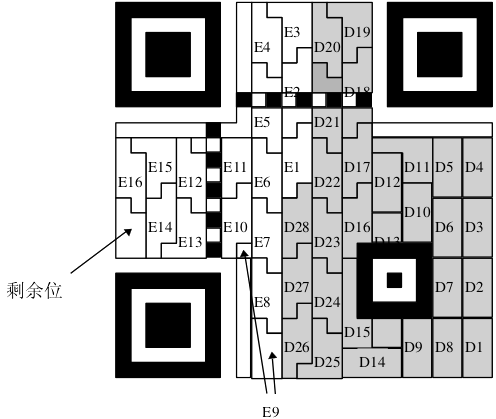
\includegraphics[scale=0.6]{figures/QR_Word.png}
\caption{二维码码字排布}
\end{figure}

QR码支持编码纯数字、数字与字符混合编码、8位字节码和包含汉字在内的多字节字符编码。除了8位字节码无压缩直接保存,其余内容都会进行压缩以增加存储容量。为保证传输的高效性,在本系统中,由于传输内容是比特流,不存在多字节字符的中国汉字与日本汉字内容,因而编码侧不会进行多字节字符的编码,解码侧也无需进行多字节字符的解码。如果使用多字节压缩,系统会因为字库原因产生数据丢失。

在国际标准二维码(以下简称ISO二维码)中,每一个码字都可以存放不同编码的内容,而二维码的容错也是由码字作为定义标准的。也就是“H级别容错最多可以允许30\%的码字发生错误”而不是“H级别容错最多可以允许30\%的码元发生错误”。在本项目的应用场景中,鉴于传输的均是8bit字节数据,并且传输的错误会随机的散步在整个二维码中,导致了30\%的码字错误率落实到码元上只能容许10\%左右的错误,在极端情况下,5\%的码元错误率会引起80\%的码字都发生错误,这是不可被接受的。因此,在编码模块中我们修改了纠错部分的定义,去除了码字概念,直接在原始的二进制数据上使用ISO二维码相同的里德-所罗门算法对信息进行编码,使得系统的可靠性有了较大的提升。

删除ISO二维码所定义的码字概念,在原始的写入数据上直接进行基于GF8的里德所罗门纠错,将纠错的数据追加到原始数据尾部。随后依照ISO/IEC 15415:2011规定的二维码写入方式,将编码后的数据写入到二维码中,可以使得二维码的纠错摆脱码字限制,回到初始的码元定义,更加符合本项目的工况。

\section{图像二值化与平滑边缘}

为了准确的获得二维码解码所需的格点信息,需要将二维码进行二值化处理以便于算法进行突变边缘的判断。

由于摄像头不可避免的存在无法即时消除的暗角,全图的亮度并不统一,没有单一的硬阈值可以使二值化有良好的效果。在正常情况下,背景和二维码目标的区分是明显的,照度是均匀的,只需要简单地使用全局二值化方法即可,常见的方法有固定阈值法、大津法、直方图双模阈值法等。在光照不均匀的情况下,这一点并不适用,固定阈值会导致全局亮度不平衡,无法正确解码,所以需要采用自适应局部阈值法来处理。

局部自适应阈值法根据每一个像素的邻域的像素值分布来确定该位置像素的二值化阈值。这样做的好处是每个像素位置的二值化阈值不是固定的,而是由周围区域的像素分布决定。一个像素的邻域如果亮度较高,那么它会被赋予较高的二值化阈值,而亮度较低的图像区域则会被赋予较小的二值化阈值。这样做可以能使得亮度不均匀的图像可以以一种较低成本的方式获得较好的二值化结果。本项目采用局部邻域块的算数平均值作为局部二值化的阈值,在有较好的效果的情况下所花时间较短。

采用局部自适应二值化,为每一个区块赋予不同的阈值,以求达到较好的二值化效果。二值化后每个像素点的值参考预期自身最近邻的k个像素点的平均亮度得到。具体可参考下式:

$$
lum_{i,j}=0.299pix_{i,j}[0]+0.587pix_{i,j}[1]+0.114pix_{i,j}[2] \geq \sum_{i-c}^{i+c}L(pix_{i,j})\quad?\quad 255\quad : \quad 0
$$

在实际应用中,对于每一个像素点都进行如上式的运算所需的时间成本是不可接受的,因此在实际应用中,采用了分块阈值的方法,将原始图像分为了一系列的网格区域,对每个区域计算平均明度,并对网格内部赋予该值作为二值化阈值。

对于二值化之后的二维码,采用了快速滑动窗口滤波,消除了局部的毛刺,为后续的检测识别流程提供了基础。快速滑动窗的实现参考下式:

$$
lum_{i,j}= (pix_{i,j} == pix_{i-1,j}\quad \&\quad pix_{i,j} == pix_{i+1,j})\quad?\quad 255\quad : \quad 0
$$
$$
lum_{i,j}= (pix_{i,j} == pix_{i,j-1}\quad \&\quad pix_{i,j} == pix_{i,j+1})\quad?\quad 255\quad : \quad 0
$$

\section{二维码格点识别}

由二维码的寻像图形与校正符推理得到二维码数据块之间的偏移量(一阶差分)与偏移量变化(二阶差分),线性偏移即可得出只发生梯度变化时每个模块的位置。

由于摄像头与屏幕之间的位置限制,必须采用球面镜头进行拍摄,使得最终得到的画面会发生鱼眼形变。在项目中,尝试过基于摄像机与镜头内参的鱼眼矫正方法,但效果不能令人满意。摩尔纹也对项目造成了影响\cite{zhang2022mobiscan}。原始图片以及基于线性推移算法得到的结果如图3.2与图3.3所示。

\begin{figure}[!htbp]
\centering

\includegraphics[scale=1]{figures/QR_Cap_00.png}
\caption{二值化后的二维码}
\end{figure}
\begin{figure}[!htbp]
\centering

\includegraphics[scale=1]{figures/QR_Cap_GF.png}
\caption{错误的格点识别结果}
\end{figure}

不难看出,算法返回的格点中心位置与实际的格点中心位置存在一定偏移。这会对后续的解码算法造成非常显著的影响,因为格点识别的准确率会直接影响最终的信息解码率。为了解决线性变化与非线性变化,在固定二阶差分偏移的基础上,每一个生成的点需要主动的感知其在空间中的位置,及时的对二阶差分产生的误差进行矫正。为此,项目实现了一套基于专家系统的自感知格点校正系统。具体流程由下例以及图3.4到图3.13阐释。

第一步,获取先验知识,由先前得到的点序列求出平均偏移向量。

\begin{figure}[!htbp]
\centering
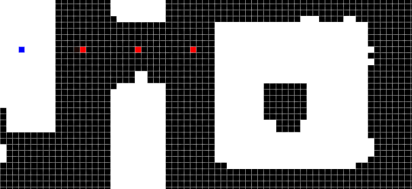
\includegraphics[scale=1]{figures/QR_Prf/图片1.png}
\caption{步骤一}
\end{figure}

第二步,根据先验知识,线性推算下一个点的坐标。

\begin{figure}[!htbp]
\centering
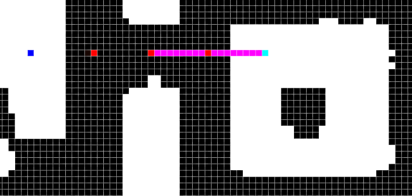
\includegraphics[scale=1]{figures/QR_Prf/图片2.png}
\caption{步骤二}
\end{figure}

第三步,确定扫描方向,在最边缘一圈的点无需进行某些方向的扫描,因为不会得到结果。由于这一点为图像中任意一点,故需要进行四个方向的探测。

\begin{figure}[!htbp]
\centering
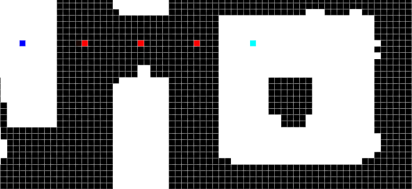
\includegraphics[scale=1]{figures/QR_Prf/图片3.png}
\caption{步骤三}
\end{figure}

第四步,向上探测,获取最近邻突变点坐标。

\begin{figure}[!htbp]
\centering
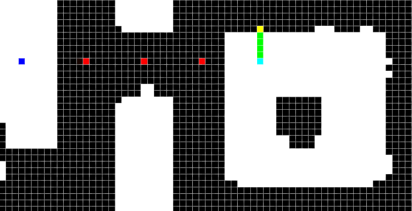
\includegraphics[scale=1]{figures/QR_Prf/图片4.png}
\caption{步骤四}
\end{figure}

第五步,向下探测,获取最近邻突变点坐标。

\begin{figure}[!htbp]
\centering
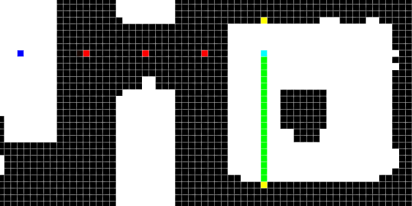
\includegraphics[scale=1]{figures/QR_Prf/图片5.png}
\caption{步骤五}
\end{figure}

第六步,依据上下突变点坐标、距离,参考先验的平均偏移向量,重新计算自身的y轴坐标。

\begin{figure}[!htbp]
\centering
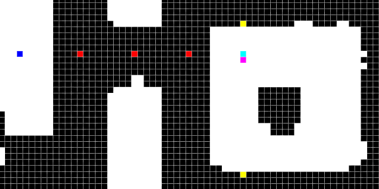
\includegraphics[scale=1]{figures/QR_Prf/图片6.png}
\caption{步骤六}
\end{figure}

第七步,移动扫描起点。

\begin{figure}[!htbp]
\centering
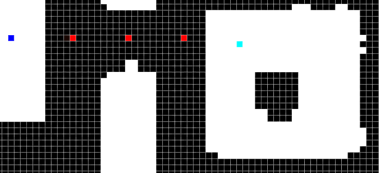
\includegraphics[scale=1]{figures/QR_Prf/图片7.png}
\caption{步骤七}
\end{figure}

第八步,向左探测,获取最近邻突变点坐标。

\begin{figure}[!htbp]
\centering
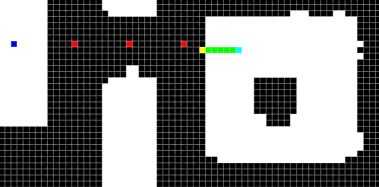
\includegraphics[scale=1]{figures/QR_Prf/图片8.png}
\caption{步骤八}
\end{figure}

第九步,向右探测,获取最近邻突变点坐标。

\begin{figure}[!htbp]
\centering
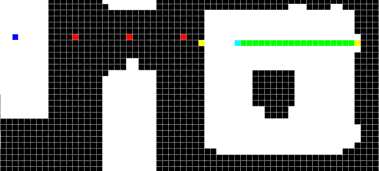
\includegraphics[scale=1]{figures/QR_Prf/图片9.png}
\caption{步骤九}
\end{figure}

第十步,依据左右突变点坐标、距离,参考先验的平均偏移向量,重新计算自身的x轴坐标。

\begin{figure}[!htbp]
\centering
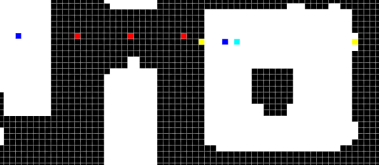
\includegraphics[scale=1]{figures/QR_Prf/图片10.png}
\caption{步骤十}
\end{figure}

由此,可以更为准确的获得自身的位置坐标。此外,基于点对之间的位置关系,可以进行基于最近n个点的移动平均校正,将少数偏移点的位置进行校正与恢复。基于专家系统的自适应格点识别算法结果如图3.14所示。

\begin{figure}[!htbp]
\centering

\includegraphics[scale=1]{figures/QR_Prf/图片11.png}
\caption{正确的格点识别结果}
\end{figure}

\section{基于位置缓存的二维码加速识别}

为了实现高速的二维码识别,针对二维码位置不变的特点,本项目软件部分设计了二维码位置缓存私有解码算法,可使二维码解码速率大大提升。

二维码的识别过程首先进行的是寻像图形的定位,根据辅助定位块进行偏移纠正,而后读取版本信息,根据偏移量获得每次一个二维码信息块的位置。这一过程往往通过遍历完成,在一个高分辨率的图像中进行这样的遍历过程是非常耗时的。

由于摄像头与屏幕的相对位置不发生变化,二维码在屏幕中的位置也不发生变化,因此上述的定位过程在实际执行时,每次返回的都是相同的结果。利用这一点,可以在后续的识别过程中使用之前的定位结果,跳过长耗时的处理流程,达到加速解码的目的。二维码加速识别的流程如下图所示:

\begin{figure}[!htbp]
\centering
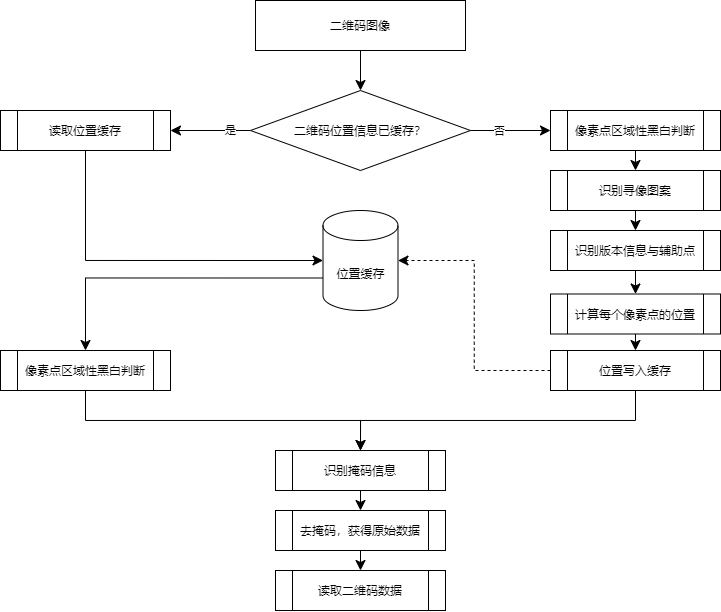
\includegraphics[scale=0.5]{figures/QR_Prf/QR_Fast.png}
\caption{二维码加速识别}
\end{figure}

为了防止错误的位置缓存对二维码的识别结果造成影响,二维码的位置缓存也有自身的刷新模式,分为定时刷新与触发刷新。在定时刷新模式下,每隔给定的Interval帧重新初始化一次格点,当Interval为0时,退化到没有位置缓存的情况。在触发刷新模式下,位置缓存会捕获自身的环境变量来尝试了解后续解码的情况,当连续Counter帧都不能成功解码时,重新初始化一次格点。

\section{基于机器学习的色彩分类}

暗角效应与色彩混叠会对颜色识别造成巨大干扰。直接采用得到的彩色图像效果会引起非常低质的解码结果。为了抵消在成像环节产生的干扰因素,需要在获取彩色图像的基础上进行包括暗部补偿(消除暗角效应)、色彩校正与白平衡的一系列图像处理操作,尽可能还原原始图像。摄像头捕获到的原始图像如下图所示。

\begin{figure}[!htbp]
\centering
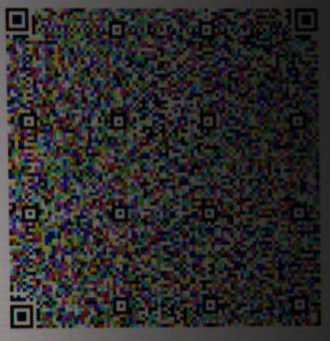
\includegraphics[scale=1]{figures/QR_Cap_RAW.png}
\caption{拍摄到的二维码图像}
\end{figure}

白平衡是一个描述屏幕中红、绿、蓝三原色混合产生的白色的准确性的指标。白平衡是一个非常重要的概念,可以用来解决一些色彩再现和色调处理问题。其基本概念是:"白色物体无论在何种光源下都能再现为白色",在某一特定光源下拍摄时发生的任何色差都可以通过放大相应的补色来进行补偿。通过白平衡补偿,我们可以在一定程度上消除画面的整体色彩偏差。\cite{陈申渭2019摄屏类图像重构算法}

暗角是由于镜头系统的光学特性而在摄影图像中观察到的径向亮度下降。在数字摄影中,相机传感器的方向性灵敏度曲线进一步增加了这种影响。在\cite{zheng2008single,lopez2015revisiting}中介绍了一种新的方法,用于对单一图像中的暗角进行免校准的追溯校正,将信息最小化的概念应用于暗角校正,使用对数强度熵作为一种具有卓越收敛特性的强度伪影校正的缩放不变量信息测量。其次,一个受限的径向多项式消隐函数确保了单调的强度曲线。由此产生的消光算法在计算上是非常高效和稳健的,基于此方法可以有效的减少暗角效应对于结果的影响。

在完成色彩的初步恢复之后,需要进行通道分离,将RGB色彩空间的图像转变为八分类或是三个二分类的一个结果,完成原始二维码数据的提取。

\begin{figure}[!htbp]
\centering
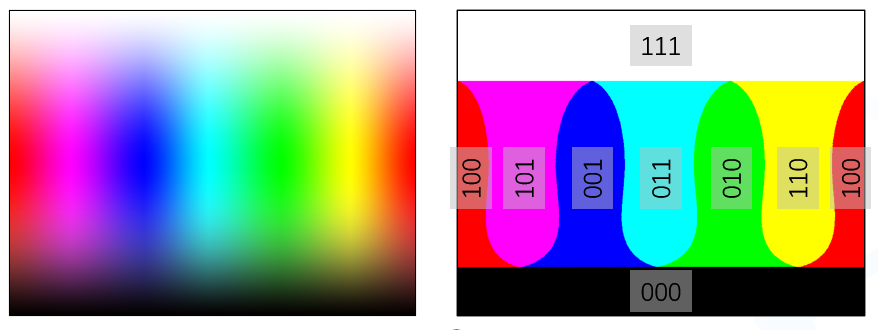
\includegraphics[scale=0.5]{figures/Color_Sp.png}
\caption{基于阈值的二维码色彩分类}
\end{figure}

基于采集得到的图片,即使是在完成了上述的各种修复流程后,也不能直接依靠阈值对色彩进行区分。在不同的图像区域,视周边颜色的不同,同一种基础色会发生较为严重的色彩偏移。加之拜耳阵列相机对于色彩混叠区域的色彩还原本身就有一定的欠缺,因此需要其他工具的引入。

\begin{figure}[!htbp]
\centering
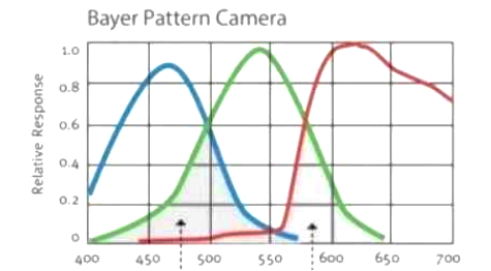
\includegraphics[scale=0.8]{figures/Color_Ba.png}
\caption{拜耳阵列相机颜色响应曲线}
\end{figure}

在本项目中,受到论文\cite{yang2018robust}的启发,使用一个SVM或逻辑斯蒂回归器进行色彩的直接8分类,利用统计学原理获得最大概率似然输出。

\begin{figure}[!htbp]
\centering
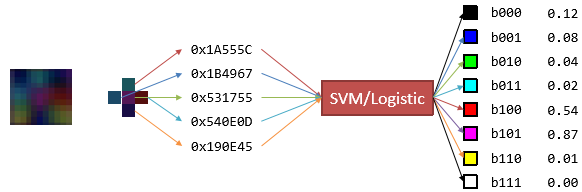
\includegraphics[scale=1]{figures/Color_Lo.png}
\caption{机器学习二维码色彩分类流程}
\end{figure}

采集了250万条清晰的数据样本,每个样本包含二维码信息块中心像素的颜色以及其最临近的8个二维码信息块中心像素的颜色,共9个RGB融合为一个27维向量作为分类器输入,8分类的置信度作为分类器输出。在构建的测试集上准确率可以达到98.6\%。在实际使用场景中,由于系统不同步带来的拍摄问题,可能会有画面刷新不完全等因素,造成准确率的下降,但总体准确率在85\%以上。

\section{基于二维码的数据传输协议MTPOQ}

MTPOQ(Message Transmission Protocol Over QR-Code,基于二维码的信息传输协议)是本项目设计中为了完成数据在二维码信道上进行无差错传输而设计的专用私有数据传输协议。

\begin{table}[htb]
  \centering
  \begin{minipage}[t]{0.8\linewidth} 
  \caption[MTPOQ组成]{MTPOQ组成}
  \label{tab:template-files}
    \begin{tabularx}{\linewidth}{lX}
      \toprule[1.5pt]
      {\heiti 字段名} & {\heiti 描述} \\\midrule[1pt]
      SN    & [2Byte] 任务序列号 \\
      PN    & [2Byte] 分包偏移量 \\
      TP    & [2Byte] 总发包数量 \\
      Data  & [不超过二维码上限] 传输数据内容 \\
      CRC   & [2Byte] CRC16校验码 \\
      EOF   & [3Byte] 固定尾部标识\\
      \bottomrule[1.5pt]
    \end{tabularx}
  \end{minipage}
\end{table}

协议主要包含以下部分:

任务序列号:区分多个在二维码信道上同时传输的任务唯一标识;

分包偏移量:二维码携带字段在传输数据整体的偏移量;

总发包数:任务含有的二维码数量;

校验码:校验采用CRC校验数据有效性;

尾部标识:提示二维码的数据结束,兼做数据校验。

为保证经过二维码信道的数据的有效性,需要实现无差错传输,因此对所有出现错误的二维码解码数据都必须丢弃。二维码自身具有一定的抗干扰与纠错能力,出于安全性与可靠性考虑,本系统选择在二维码自身的检错纠错基础上进行额外的差错检测。

发送方计算机使用一个公式计算出要传输的数据中所包含的信息值,并将这个值追加到要传输的数据中,而接收方计算机用相同的公式对去掉CRC的受到的数据进行同样的计算,如果传输过程中没有错误发生,那么应该得到相同的结果。如果这两个CRC结果不一致,则说明传输中出现了错误。

在MTPOQ协议中设置了多个字段以进行无差错传输。

1、EOF尾部标识校验:对尾部标识非预期的包进行丢弃。

2、Data长度校验:对超过预期长度的包进行丢弃。

3、偏移量校验:对偏移量大于总发包数的包进行丢弃。

4、CRC校验:对无法通过CRC(循环冗余校验)的包进行丢弃。

具体数据有效性校验流程如图3.20所示。

\begin{figure}[!htbp]
\centering
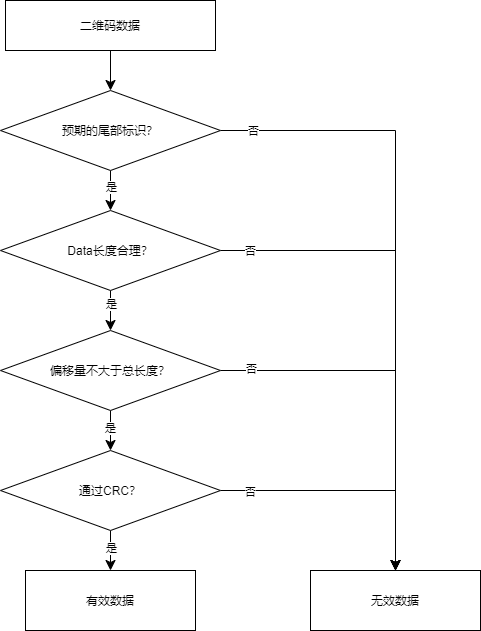
\includegraphics[scale=0.6]{figures/CRC_Check.png}
\caption{数据校验流程}
\end{figure}

\section{本章小结}

本章介绍了一种复杂环境下的高效自适应二维码编解码方法,在已有研究的基础上对部分算法进行加工、合并,针对本项目对已有的技术做出了针对性的改进。创新性的提出了二维码的位置缓存解码方案、自适应的高精度格点识别方法、基于逻辑斯蒂回归的色彩分类模型以及基于二维码的数据传输协议,实现了针对这一特殊场景下在速率与可靠性较ISO二维码远高的自定义二维码及其编解码方案。
% !Mode:: "TeX:UTF-8"
\mychapter{基于二维码的图像识别单向传输系统}
\label{cha:sys}

基于上文的复杂环境下的高效自适应二维码编解码,现在我们有能力在屏幕-摄像机的物理信道上构建真正的逻辑传输信道,从而实现本项目要求的单项文件传输隔离系统。本章主要着重于软件层面,介绍在物理设备上构建单向传输系统的实现过程及其细节。

\section{软件整体架构}

本项目采用Rust,C与C++语言开发,二维码的编码采用Rust的QRCode-Rust, 解码采用Bar-Decoder,均基于本项目的使用场景做了特异性优化与改进;多线程采用RUST原生线程实现构建线程池;进程间通信采用ZeroMQ。系统运行于Ubuntu 20.04系统中,Rust使用采用Version 2018。

\subsection{流程架构}

图像识别单向隔离装置技术架构从下到上分为五层,分别为:物理层、编解码层、数据封装层、数据链路层和网络接口层,包括服务和协议有:二维码编码服务、二维码解码服务、MTPOQ传输协议、数据发送服务、数据接收服务、高安全级网络接口、低安全级网络接口。各个层次的上层依赖于下层具体实现,但又逻辑上相互独立,具有较好的可扩展性。图像识别单向隔离装置技术架构如图4.1所示。

\begin{figure}[!htbp]
\centering
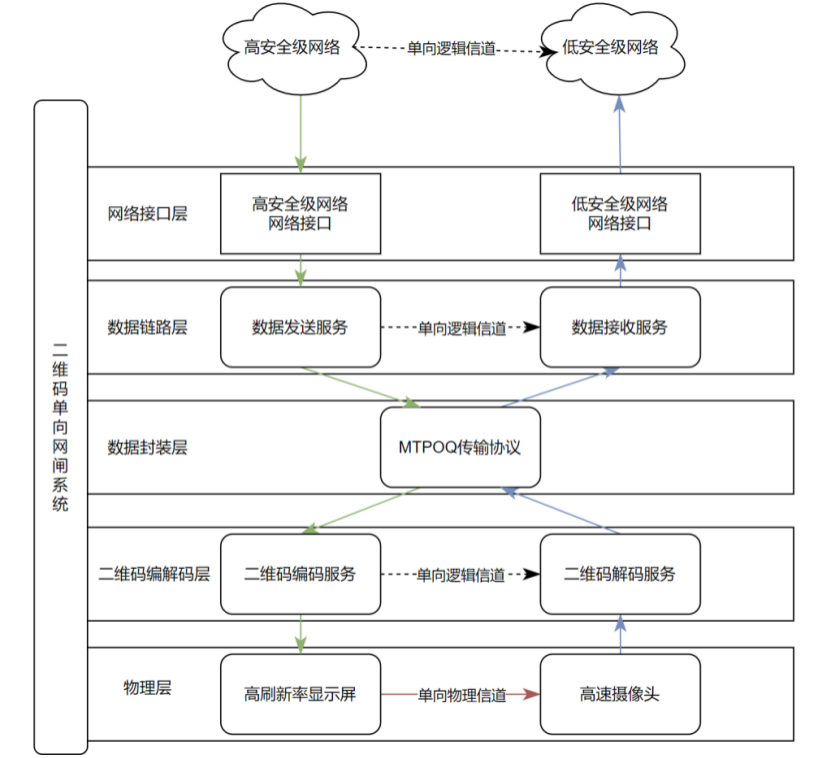
\includegraphics[scale=0.6]{figures/SStructure.png}
\caption{图像识别单向隔离装置技术架构}
\end{figure}

最底层为基于显示器与摄像头的物理单向信道。在高安全级的网络端放置一个网络数据包编码器和一个屏幕,在低安全级的网络端放置一个摄像头和一个网络数据包解码器。如此一来,由于网络包信息可以被编码为二维码展示在屏幕上而被摄像头捕获到,高安全级数据可以流向低安全级网络;由于摄像头不可能向屏幕传播任何信息,则低安全级网络中的数据不能流向高安全级网络。

二维码编解码层包括二维码编码服务与二维码解码服务。编码服务提供了高效、准确的将数据编码成为二维码能力,解码服务提供了二维码解码服务。编码服务与解码服务共同构成了二维码传输信道的数据传输实现。

数据封装层所提供的MTPOQ数据报构成了二维码的内容,也是数据抽象的重要形式无论所传输的数据是什么,协议栈都会将其作为二进制流对待。通过封装成为MTPOQ数据报可以实现数据的透明传输,其本身所携带的额外信息为上层实现检错提供了可能。

数据链路层包括数据发送服务与数据接收服务。数据发送服务将接受自上层的任务序列进行分包、封装成帧后交由下层传输,数据接收服务将下层交付的数据报进行校验、组装后提交到上层。基于MTPOQ与二维码,在数据链路层可以实现数据的无差错传输。

网络接口层提供由一般网络使用的TCP/IP协议到内部传输协议的相互转换,以免去通过本系统进行数据传输的外部开销。

针对实现基于二维码图像识别的单向隔离装置这一目标,需要一系列模块提供服务支持由普通网络数据到模块内部专有数据,再转换到普通网络数据的这一过程,以实现数据在二维码图像识别单向隔离装置上的传输。本系统是完整的单向传输系统,主要特色为基于光学的单向数据传输。系统组成模块如图4.2所示。

\begin{figure}[!htbp]
\centering
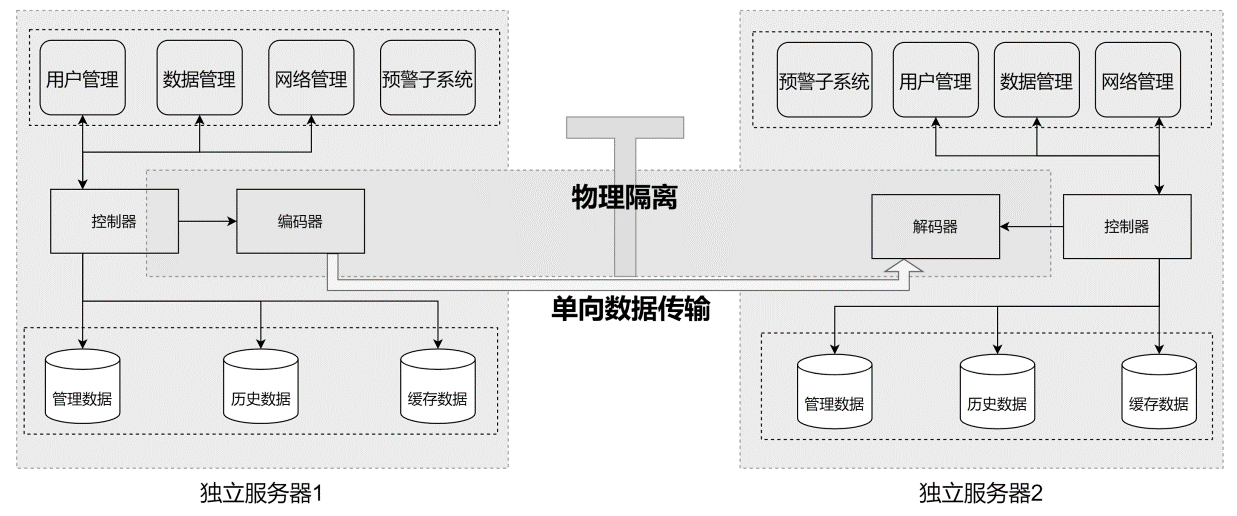
\includegraphics[scale=1]{figures/SModule.png}
\caption{系统组成模块}
\end{figure}

本系统基于二维码进行图像识别,实现数据到图像再到数据的转换。二维码的编解码速度、质量对整个系统的传输带宽至关重要。系统工作原理的大体流程如图4.3所示。

\begin{figure}[!htbp]
\centering
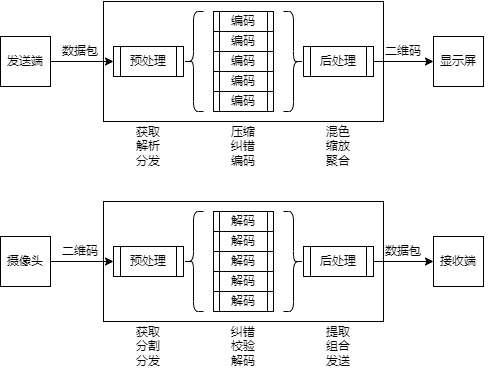
\includegraphics[scale=1]{figures/SMapReduse.png}
\caption{系统组成模块}
\end{figure}

在发送端:
\begin{itemize}
\item 编码端从上位机截获网络封包,解析应用数据;
\item 处理单元对数据进行压缩编码,然后进行纠错编码,得到图像信道数据;
\item 基于最终数据构造矩阵,形成二维编码图像;
\item 在图像信道(显示屏)上显示。
\end{itemize}

在接收端:
\begin{itemize}
\item 通过摄像机拍摄到图像,定位并分割获取图形;
\item 处理单元将图形转化为像素矩阵,识别格式和版本信息;
\item 恢复数据和纠错码,通过纠错码进行校验和纠错,得到原始网络封包;
\item 网络封包聚合后,发向接收端的传统网络信道。
\end{itemize}

\subsection{技术架构}

通过C与C++调用摄像头的API获得拍摄图片。C语言是一种广泛使用的专业语言,拥有非常高的执行效率,适合从摄像头高速获取采集到的图像数据。

软件核心编码层使用Rust语言开发。Rust语言于2010年推出,其开发的主要目的是提高整体安全性,提供优秀的模块化、良好的并行性和性能。其语言设计逻辑和本项目追求高安全、高并发和高性能的目标相吻合。Rust语言具有一系列的优秀特点,包括:不编译有错误的代码,绝佳的执行速度,硬件级代码,垃圾回收与内存安全,低成本的抽象。

操作系统使用基于Ubuntu的安全加固的Linux自制系统。针对系统安全性的措施包括了取消所有服务器的root远程ssh登录,限制su-root的用户权限,同时ssh登录端口调整,外网ssh登录全部调整;Iptables禁止除单向网闸服务外的网络权限,防止旁路资源被利用;调整密码过期时间和复杂度;调整网络泛洪、SYN等防攻击策略参数;清理服务器无效账户如Ip、news等,调整系统关键目录权限;优化服务器连接数参数;日志管理:登录认证记录等。

ZeroMQ(简称ZMQ)是一个简单易用的传输层,是一个类似于套接字库的框架,使套接字编程更简单、更干净、更强大。ZMQ提供了一个简单的套接字API,通过后台的I/O线程进行消息路由,提供多种模式的消息传输,异步地读写消息。当一个节点被移动或掉线时,ZMQ会自动连接或重新连接。\cite{郑帅2014基于}

采用国密SM4.0加密算法进行数据加密。SM4.0是中华人民共和国政府采用的一种分组加密标准,由国家密码管理局于2012年发布。组长和密钥长度均为128比特,加密算法和密钥扩展算法采用32轮的非线性迭代结构,S-box为固定的8位输入和8位输出。国密SM4.0加密算法流程如图4.4所示。

\begin{figure}[!htbp]
\centering
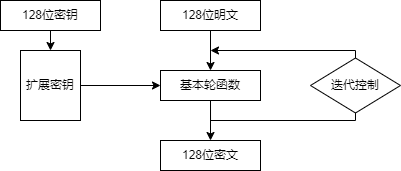
\includegraphics[scale=0.8]{figures/SM4.png}
\caption{国密SM4.0加密算法}
\end{figure}

\section{二维码编码}

二维码编码服务实现从编码队列中提取数据包,多线程地进行高速编码,并最终将编码后的二维码展示在屏幕上。

\subsection{二维码构建}

把数据包通过冗余编码方式编码为符合标准的二维码图像,在有少量遮挡和干扰的条件下要能够被识别。将标准的二维码图像融合编码为RGB三色的二维码图像。实现将编码的二维码图像编排为合理的二维码阵列,调用显示屏接口,高速展示二维码图像阵列。

为了提升IO效率,同时增加系统的带宽,在屏幕上将会展示由8个3色二维码构成的彩色二维码阵列。也就是在每次刷新的过程中将有24组二维码数据被编码为一张图片,展示在屏幕上。

由于二维码的编码过程由CPU直接执行,因此大量的高分辨率数据对程序执行是有害的。在二维码合成的过程中,通道合成与二维码拼接均在低分辨率空间下完成,直到被展示时才会被上采样为全尺寸的二维码图像。

二维码的构成与合成如图4.5所示。

\begin{figure}[!htbp]
\centering
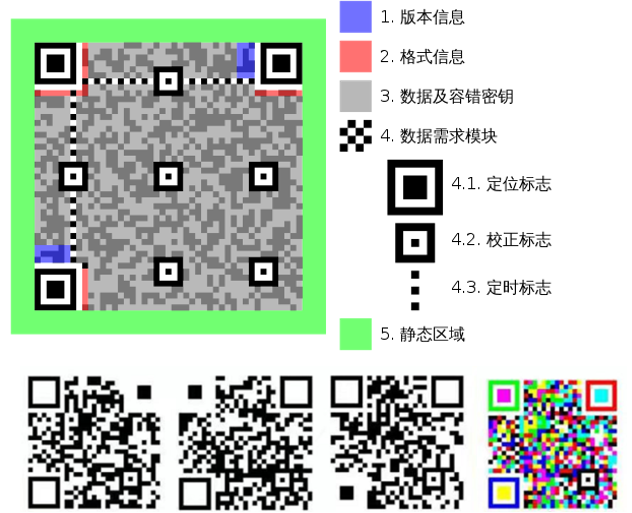
\includegraphics[scale=0.8]{figures/QR_Str.png}
\caption{二维码的构成与合成}
\end{figure}

在图像编码完成后,等待操作系统的VSYNC信号,随后通过操纵FrameBuffer将渲染完成的图像展示在屏幕上。由于显示器逐行扫描刷新的特性,需要保证显示器与系统输出的画面垂直同步以防止画面撕裂。图4.6是一个画面撕裂的例子。

\begin{figure}[!htbp]
\centering
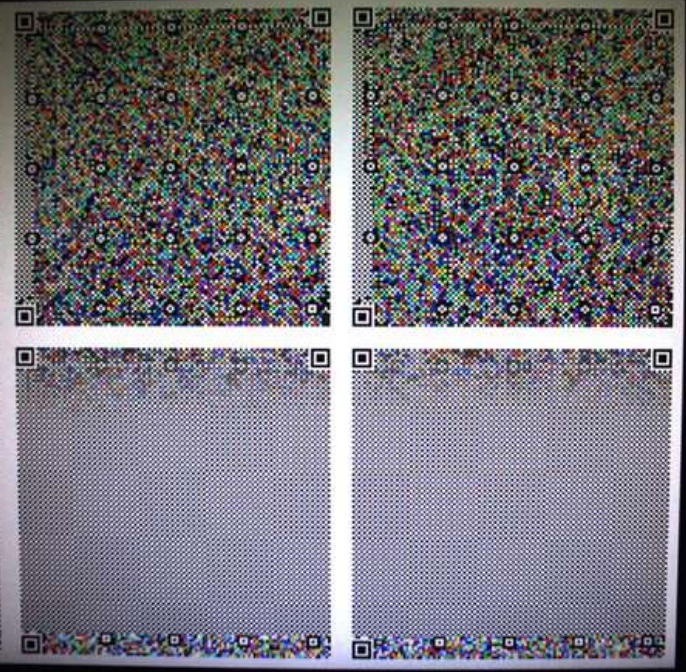
\includegraphics[scale=0.6]{figures/QR_Cap_NV.png}
\caption{发生撕裂的二维码}
\end{figure}

最终展示的效果如图4.7所示。

\begin{figure}[!htbp]
\centering
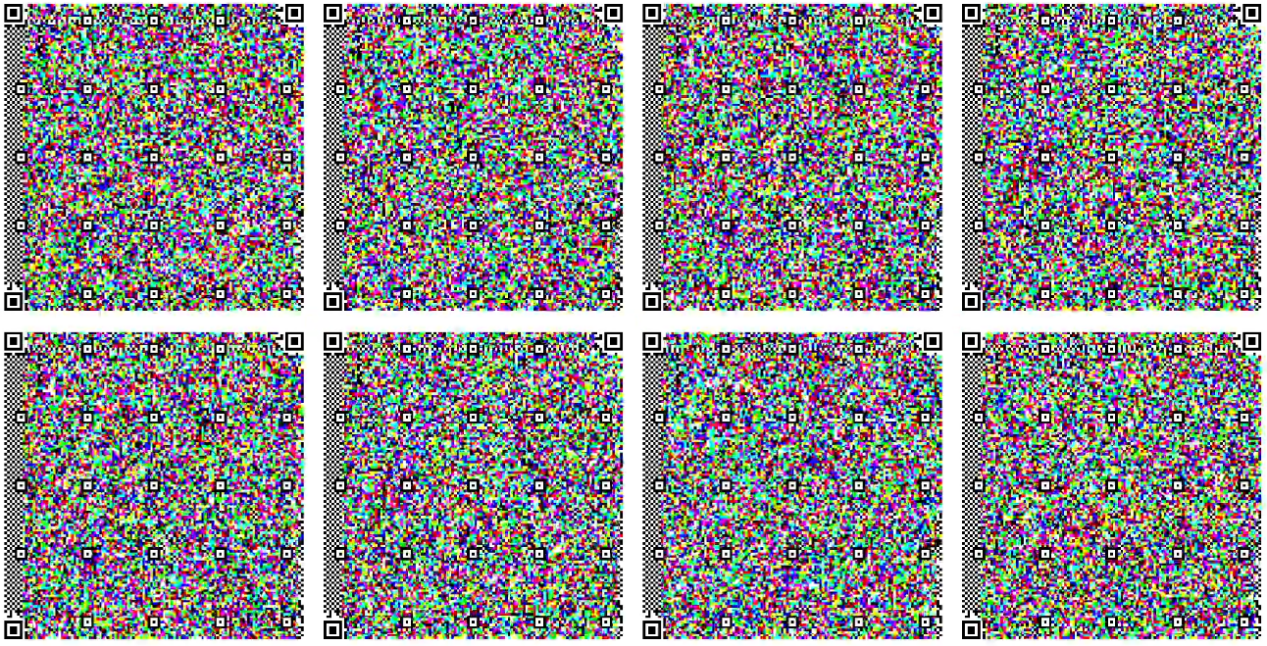
\includegraphics[scale=0.8]{figures/QR_Dp.png}
\caption{合成的彩色二维码阵列}
\end{figure}

\subsection{二维码并发编码}

为保证二维码的高速生成,需要充分利用CPU性能编码二维码,因此多线程并发不可或缺。采用线程池与队列结合的方式实现多线程并发,保证二维码的生成效率。

线程池是一组预先分配的线程,它们等待或准备处理一个任务。当程序收到一个新任务时,线程池中的随机一个线程被分配到该任务,这个线程离开线程池并处理该任务。\cite{田素贞2012基于.}然后,在该线程处理该任务时,其余的线程可以用来处理其他收到的任务。当线程处理完任务后,它返回到自由线程池中,等待新的任务并进行处理。线程池可以看做一种对于计算机资源的池化技术。具体结构如图4.8。

\begin{figure}[!htbp]
\centering
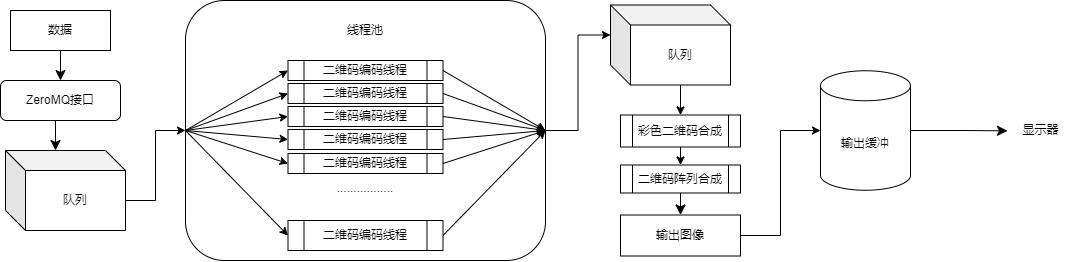
\includegraphics[scale=0.4]{figures/ENC_TP.png}
\caption{二维码线程池编码}
\end{figure}

\subsection{并发控制}

单个二维码的容量由二维码版本、纠错率与编码方式决定。受限于二维码实际用来编码数据的码元数量,单个二维码的编码容量具有上限,即不可将超过二维码容量的数据内容编码到二维码内。在发送超过单个二维码容量的数据内容时需要采取策略对数据进行分片,将超长数据编码到多个二维码中。

由于采用了线程池并发,任务的分配时机与他的完成时机不再对应,先分配的任务可能晚完成,后分配的任务也可能先完成。因此,在编入二维码的数据片段中必须有任务分段的完整位置标识。

由于图像展示逻辑只有在队列中有超过24个编码完成的二维码数据后才会被触发,因此任务片段的数量必须是24的整数倍,否则可能出现部分数据“卡死”在队列中无法被发送的情况。

\section{二维码解码}

二维码解码服务实现从二维码解码队列获取二维码,并对二维码实现精准定位,定位后分离RGB三个通道,还原为黑白通道,最后对黑白二维码进行符合协议标准的数据解码。将解码的数据包推入发射队列。

相机传感器拍摄彩色图像的方法之一是采用拜耳阵列。采用这种技术的传感器实际每个像素实际只负责感受一种指定颜色的亮度信息,需要利用反马赛克算法进行插值计算,最终获得一张彩色图像。拜耳阵列的问题之一,是在拍摄具有重复细节(即本项目中的屏幕,由于像素间存在间隙,实际存在大量重复细节)的画面时,容易产生彩色干扰信息(即摩尔纹)。而在反马赛克算法进行插值时,又会不可避免的引入色彩混叠与拉链效应,加之摄像头拍摄到的全为人工光源,实际采集到的图像与屏幕显示的图像存在较大差异。

解码服务通过摄像机API,以IPC方式,运用Request-Reply模型获得摄像机拍摄到的图片,进行解码获得二维码图片的原始数据。

对接收到的彩色二维码阵列图像,首先需要对二维码阵列进行色彩通道分离与图像区域裁切,将原始合并的(色彩通道数*阵列二维码个数)个二维码分离出来,而后逐个分别进行二维码的解码。解码测同样采用多线程并发以提高二维码解码的效率。

\subsection{二维码分割}

由摄像头拍摄到的彩色二维码阵列进行裁切,得到多个单独的二维码。在展示图片的过程中,各个二维码之间放置红色定位块来辅助进行二维码的分割。当有数据进行传输时,不显示红色定位块,兼用作跳过识别标识。

使用区块扫描法,获取连续单色区间$[(x_1,x_2),(y_1,y_2)]$,估算中心点位置,再根据估算中心进行四向线扫描,得到突变点系列$[(x_1,y_1),(x_2,y_2),(x_3,y_3),(x_4,y_4)]$,最终得到矫正后的中心点$(x_1+x_3/3+x_2+x_4/6,y_2+y_4/3+y_1+y_3/6)$。由此可得一系列分界点,依据分界点即可裁切出二维码图形。

\subsection{二维码寻像图形与矫正图像识别}

寻像图形由三个相同的位置检测图形组合构成,分别位于整个二维码的左上角、右上角和左下角。每个位置的检测图形由三个重叠的同心方块组成,包括7x7的暗模块、5x5的亮模块和3x3的暗模块。位置识别图案的模块宽度比例为1:1:3:1:1。在二维码的其他地方遇到类似图案的概率极低,并且通过二维码的掩码图案主动避免生成,因此视野中可能的二维码符号可以被快速识别。\cite{康春颖2009基于二维码技术的电子票务系统的研究}构成图像查找模式的三个位置识别图形的识别,可以精准地确定图像中符号的位置和方向。

寻像图形如下图所示:

\begin{figure}[!htbp]
\centering
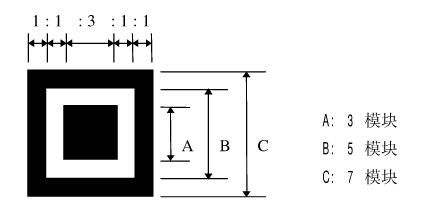
\includegraphics[scale=1]{figures/PAT_b.png}
\caption{二维码寻像图案}
\end{figure}

针对这一1:1:3:1:1的特征,使用多次穿透与模式匹配,准确获得二维码的寻像图案位置,初步推测二维码版本信息。多次穿透的方向会包括水平、垂直与主对角线方向,通过多个方向的多次穿透模板匹配,我们可以使得寻像图形中心点的绝对误差小于10\%的寻像图形长边长。基于此,我们可以准确获得二维码的寻像图案位置,初步推测二维码版本信息。
基于寻像图形的位置,我们可以指定一个范围进行模式匹配以寻找梯度校正符。梯度校正符号如下图所示:

\begin{figure}[!htbp]
\centering

\includegraphics[scale=1]{figures/PAT_s.png}
\caption{二维码梯度校正图案}
\end{figure}

由于没有计算机视觉库的支持,只能在像素空间中进行基于模板的匹配,获得校正符的位置。

\subsection{二维码并发解码}

为保证二维码的高速解码,需要充分利用CPU性能编码二维码,因此多线程并发不可或缺。采用线程池与队列结合的方式实现多线程并发,保证二维码的解码效率。

具体的实现流程与上文4.2.2节非常相似,这里不再赘述。

\section{数据发送}

在构建了二维码的编解码器后,我们即可基于二维码的编解码服务进行数据传输。本章主要内容在于说明本项目如何基于二维码进行高效率、无差错的数据传输。

在MTPOQ协议中,采用定长头部与定长尾部存放传输过程中的控制信息。原始数据作为比特流存放在数据部分中,在传输过程的任何环节都不对数据部分进行修改或访问。在编码侧,数据被分片、封装到数据报中;在解码侧,数据从数据报中被提取、组装。实现数据的透明传输。

\subsection{接收上级数据}

主线程针对物理网口,启动线程监管对于接口的连接。监管线程查询配置表,获知配置的IP、端口与协议,启动协议对应的Socket监听端口,处理到达的信息。对于UDP连接,针对到达的数据流,判断来源IP是否在白名单中,并拒绝或做接受。对于TCP连接,针对每一个TCP流,判断连接发起IP是否在白名单中,并做拒绝或启动新线程处理流。数据接收的处理流程如图4.11所示.

\begin{figure}[!htbp]
\centering
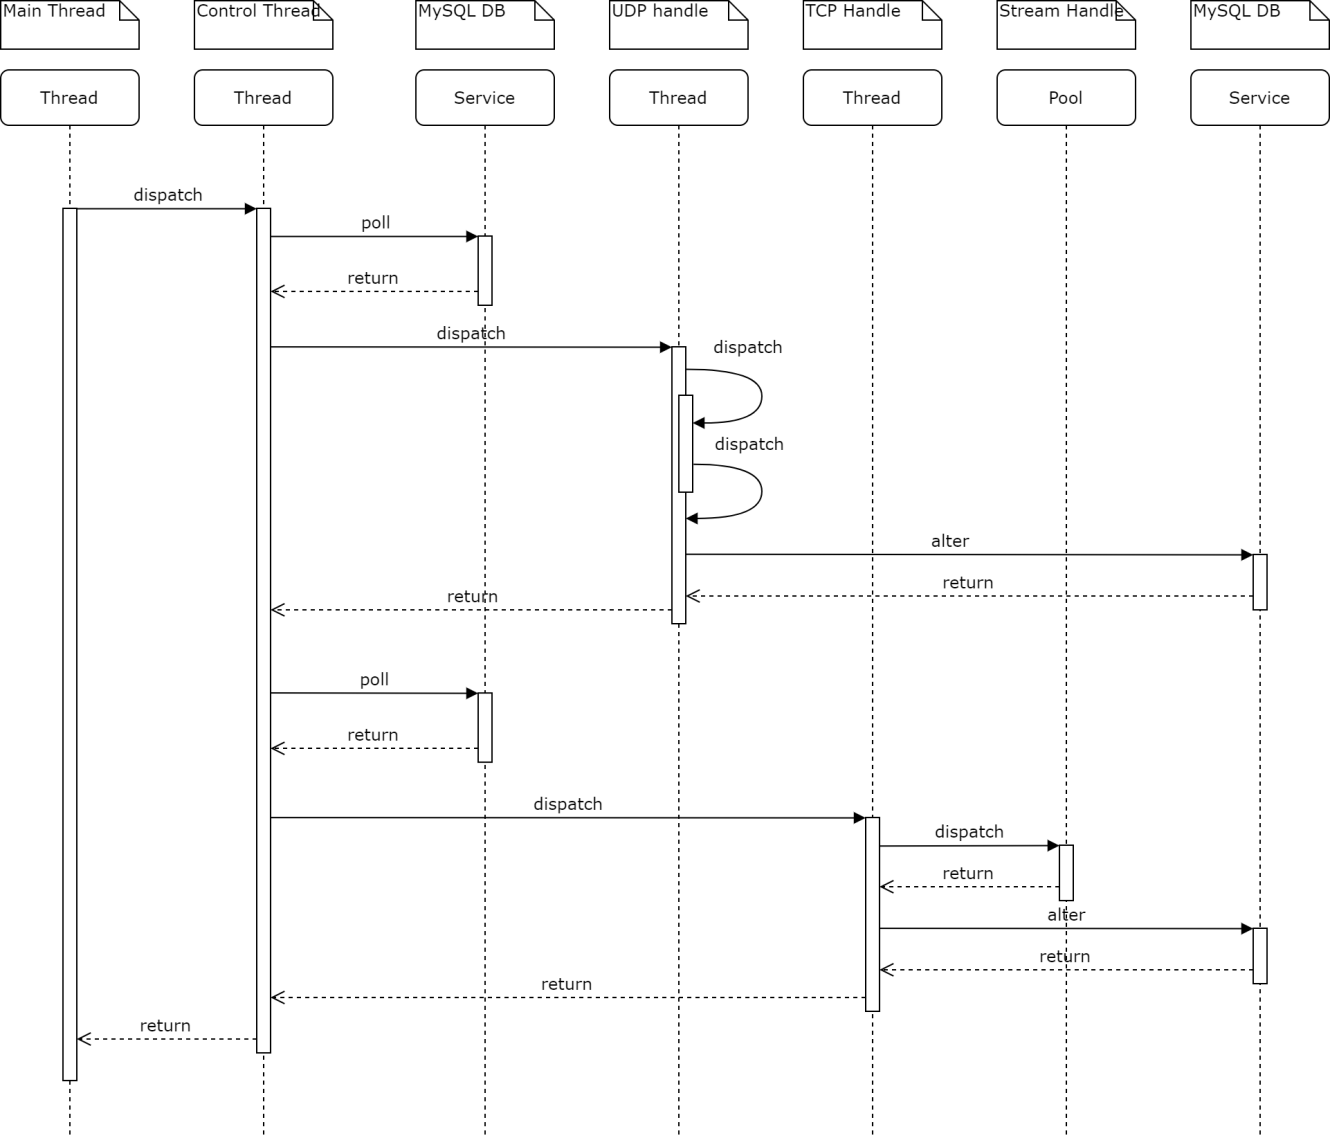
\includegraphics[scale=0.8]{figures/ST_Recv.png}
\caption{数据接收}
\end{figure}

\subsection{数据预处理}

在发送数据之前,为了传输效率考虑,我们对数据做如下的预处理:

数据流阶段。TCP是一种流协议,意味着数据以字节流的形式传递给接收者,没有"报文"或"报文边界"的概念。UDP是一个无连接协议,传输数据之前源端和终端不建立连接,当传输发生时直接将数据包发送给接收方。在数据流处理阶段,我们收集原始流式数据,获得二进制位串。

离散文件阶段。从流式数据获得的二进制位串中,解析协议内容,将数据部分缓存为文件,文件与TCP、UDP数据包内容一一对应。

文件归档阶段。TAR是Unix系统上的压缩打包工具与指令,可以将多个离散文件合并为一个归档文件,打包后的文件后缀亦为“tar”。将零散小文件组装成单个大文件,进行归档。这样做可以减少任务数量,减少大量短任务并发带来的开销。

压缩数据阶段。通过GZip对数据进行压缩编码。通过对数据进行压缩可以有效的减少文件大小,减少文件大小有两个明显的好处:一是可以减少存储空间,二是通过网络或是本项目涉及的单向网闸传输文件时,可以减少传输的时间与占用的带宽。缺点在于这将会占用编解码主机的额外算力。由于网络传输的瓶颈在于显示屏-摄像头之间传递的低效性导致的瓶颈,因此这一算力换时间的策略是值得执行的。

\subsection{数据编码}

正如同前文所提到的,单个二维码的容量有限,且我们不能保证传输信道的100\%可靠,因此,在进行MTPOQ数据的打包时,我们同时进行信源编码来提升数据的冗余度,使得最终传输的数据可以在不可靠信道上实现较高的传输成功率。在不同的MTPOQ数据包内,分散有任务的各个分片,在所有数据片段之后,我们人为的添加用于数据恢复的冗余数据片段,同样采用里德-所罗门编码,保证只要接收到足够多的正确数据就可以恢复整个任务。这一流程如图4.12所示。

\begin{figure}[!htbp]
\centering
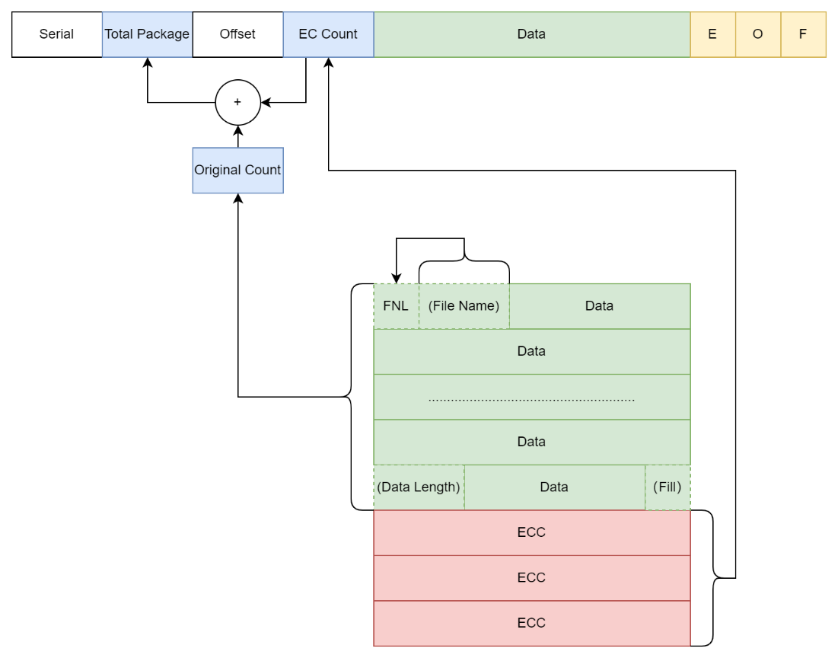
\includegraphics[scale=1.2]{figures/QR_Co.png}
\caption{数据编码}
\end{figure}

在实际传输的流程中,ECC的数量经实验,在确保99.999\%的传输可靠性的情况下,确定为:max(ceil(原始数据包数量*2 / 24) * 24, 72)。

\subsection{数据发送}

在经历前序处理流程后,将编码完成的数据通过IPC发送给二维码编码服务。数据发送服务会保证每次发送的数据包数量都向上取整到24的倍数,多余的部分由冗余度填充,以防止数据片断停留在数据管道中。流程如图4.13所示。

\begin{figure}[!htbp]
\centering
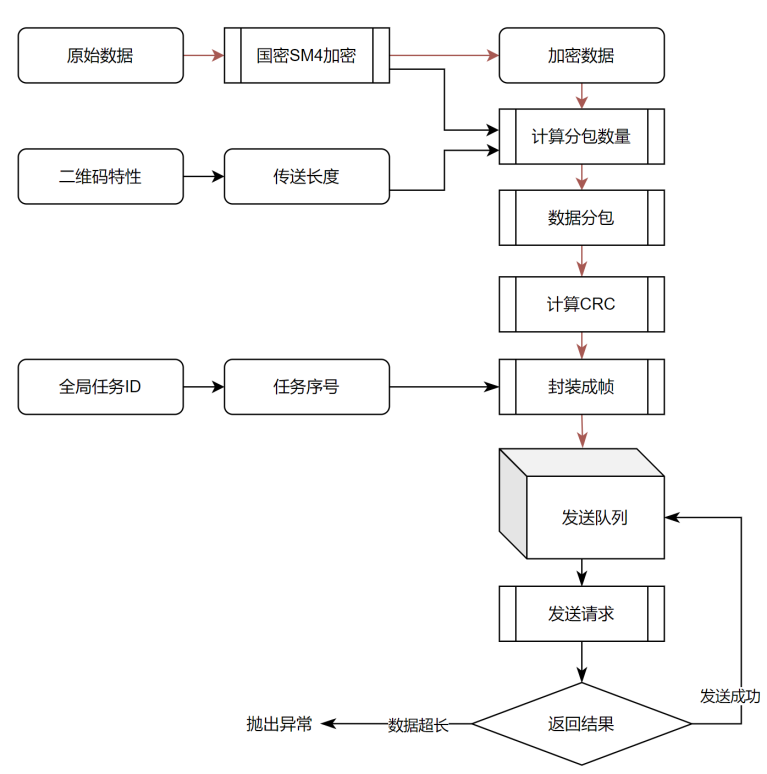
\includegraphics[scale=1.2]{figures/QR_Enc_Flow.png}
\caption{数据发送}
\end{figure}

\section{数据接收}

数据接收服务接收来自解码服务返回的MTPOQ数据报。经过数据完整性校验后,重新将分片的数据报组合为完整数据,并发送给上级组件。

\subsection{数据提取与组装}

在数据通过完整性校验而被接收后,采用[任务-分块]的二级HASH机制实现数据报片的快速、有效、离散且无冲突的临时存储。采用密码学安全的SipHash-2-4,通过让输出随机化,SipHash 能够有效减缓 Hash Flooding Attack,避免DOS的出现,保证服务的有效性。

当新任务到来时,根据序列号进行第一次HASH创建单任务数据集合,根据偏移量进行第二次HASH确定存储物理块地址,将数据报片中的数据写入内存。

任务的后续报片到来时,据序列号进行第一次HASH寻找单任务数据集合,根据偏移量进行第二次HASH确定存储物理块地址,将数据报片中的数据写入内存。

当一个任务的数据报片被全部收到时,遍历对应序列号的单任务数据集合,将离散的数据报片组装成为完整数据,之后删除任务集合中的对应序列号,释放已占用存储空间。

数据提取与组装的流程如图4.14所示。

\begin{figure}[!htbp]
\centering
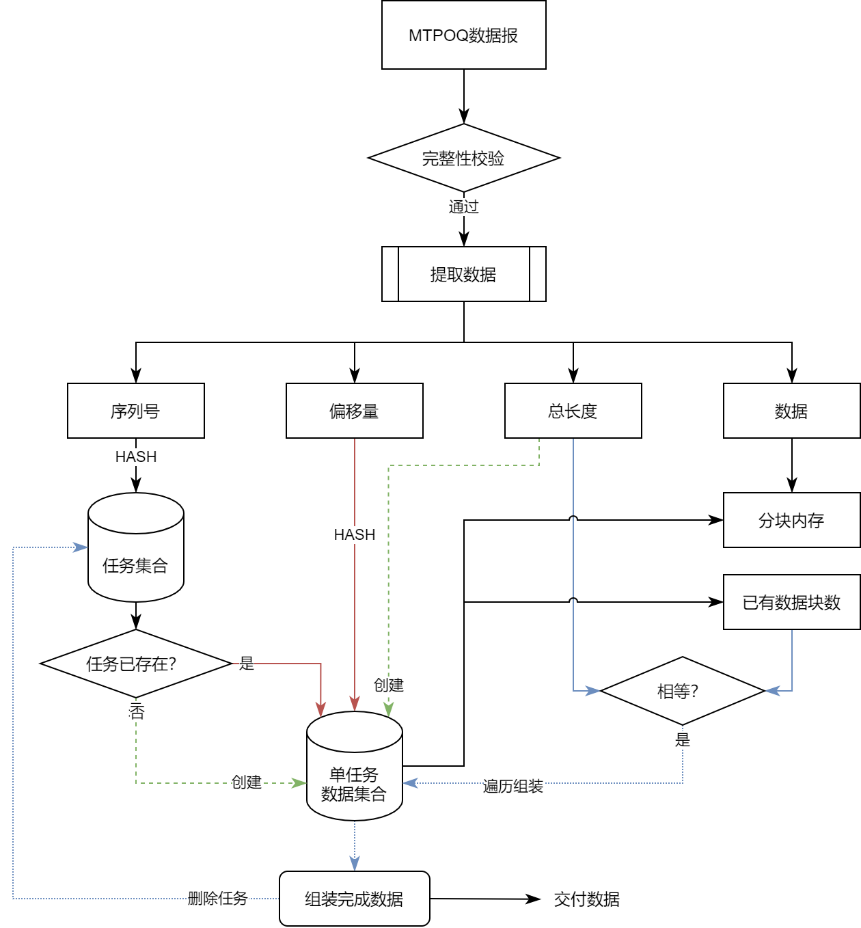
\includegraphics[scale=1]{figures/Dec_Hs.png}
\caption{数据组装流程}
\end{figure}

\subsection{数据解压缩与复原}

在发送数据时,对于一系列的TCP、UDP数据包进行了压缩打包处理以保证传输流程的高效性。在传输完成后,需要对已经压缩序列化的数据进行解包复原。此处的流程与4.4.2节为镜像关系,不再赘述。

\subsection{数据发送}

主线程接收到待发送的数据包,在数据库中查询路由表,进行协议核对,而后依照TCP与UDP分别进行处理。对UDP,直接发送到对应的目标套接字;对于TCP,尝试建立TCP连接,发送数据,然后断开TCP连接。具体流程如图4.13所示。

\begin{figure}[!htbp]
\centering
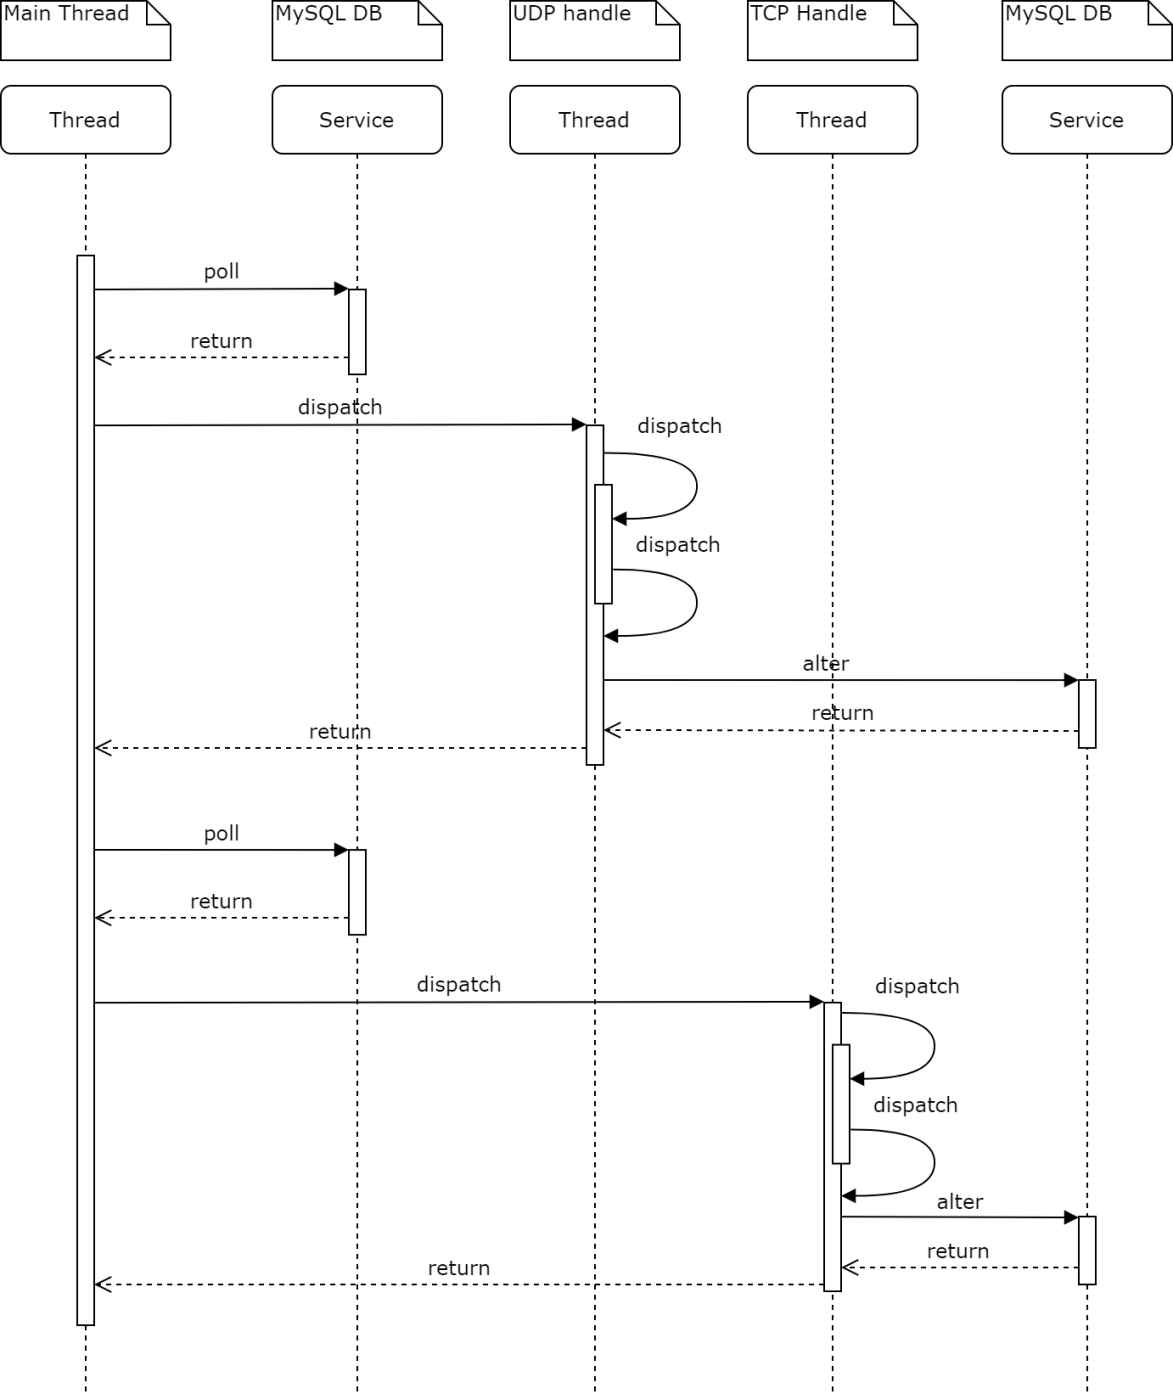
\includegraphics[scale=0.8]{figures/ST_Send.png}
\caption{数据发送}
\end{figure}

\section{数据安全性与可靠性}

对于单向网闸系统,作为网络边界管理设备,其安全性与可靠性对于整个网络系统安全可靠运行有着重大影响。针对这一问题,本项目进行了如下的实现以及优化。

\subsection{数据安全性}

实现物理隔离的通道是通过自主研发的二维码隔离通道实现的,由液晶显示器和高速摄像机组成,是本系统的核心。显示器与内部网络主机相连,高速摄像机与外部网络主机相连。内部网络主机将数据编码为二维码并显示在显示屏上。外网主通过高速摄像机机捕捉图像,进行解码,然后转发数据。物理单向隔离通道没有物理连接,确保内部和外部网络之间传输的数据的物理隔离和阻断。

采用深度定制、加固的Linux操作系统,结合内部私有协议,通过应用数据剥离、封装成图像、捕获图像、图像解码等过程,实现不同安全域之间网络数据的单向传输,从而避免系统遭受攻击与入侵。

系统将应用层的数据转换成专有的图像格式,并且对传输的数据进行安全检查,只允许安全的、可信的信息通过网闸。信息的格式、内容、时间等因素可依据用户安全策略指定。影像识别单闸对数据的交换不依赖于任何通信协议,没有建立连接会话,而是以静态的图像在内外网间传递,确保了核心应用的安全最大化。

私有的二维码协议在掩码定义、数据处理、内容分布、编码格式上与ISO国际标准二维码均不相同,内部可变参数也会更改解码的过程,外部协议无法解析私有二维码的编码内容。即使二维码图像泄露,没有协议与参数支持的情况下图像内容也无法直接解析。

\subsection{数据可靠性}

对于没有任何反馈信号、完全单向传输的物理隔绝单闸,接收端到发送端没有反向的控制帧协议,不知道对方的工作状态,不知道通信链路是否可用,无法协商双方的通信速率,发送端无法知道接收端是否准备接收数据,数据是否传输正确,不知道接收端是否正在接收数据,是否及时处理收到的数据,无法进行实时的流量控制。从理论来说,物理隔绝的单向网闸做不到绝对的可靠传输(即不重复,不遗漏,不乱序,不错误)。物理隔绝单向网闸所能做到的是尽最大可能的无差错传输,由此延长平均故障时间,提高可靠性。

二维码编码具有纠错能力。在二维码的每个数据段内散布数据与恢复内容,可以在解码同时对数据进行有限恢复,提高解码的有效性。

使用信道编码技术,利用编码方法,接收端不仅能对接收的数据进行错误检测,当检测出错误后能对错误进行定位,从而进行自动纠正。对于一个传输任务,只要接收到了足够多的正确信息,则总是可以将数据内容恢复出来\cite{杨云江2004一种在网络通信中自动纠错算法的研究}。

对传输完成的数据内容进行校验。原始的传输内嵌CRC16校验码,可以快速而有效的判别传输任务的有效性,对错误的任务进行丢弃。

\section{本章小结}

在本章,我们基于上一章所提到的二维码编解码算法,在物理硬件上实现了一条单向的、无需反向控制信息的、可以实现无差错传输的逻辑单向信道,并且有着较高的传输速率以及可靠性。由此,我们可以通过文件摆渡的方式在两个隔离的网段之间单向的传输信息。在传输文字信息的情况下,经过压缩,传输速率可以达到24Mbps,基本可以覆盖工控网络的信息流量。
% !Mode:: "TeX:UTF-8"
\mychapter{适用于二维码单向传输的硬件以及环境系统}
\label{cha:hd}

本章主要阐述与上一章所实现的基于二维码的图像识别单向网闸的配套硬件及其控制组件与用户界面的介绍。

\section{硬件设计}

硬件设计是本系统的基石。设计要求采用图像识别的方法,涉及到一个编码端和一个解码端。由于是基于摄像头拍摄屏幕这一工作流程进行实际的数据传输,要求物理设备具有很高的稳定性,物理结构必须经过精心设计,且最终成品必须容纳在标准机柜内。

\subsection{显示屏}

编码端的显示屏用于展示编码后的二维码。显示屏的刷新频率不得低于60FPS;响应时间不得高于5ms。显示屏与编码服务器之间采用可靠的有线方式连接,采用HDMI或者DP线缆以提供足够的显示带宽以支持屏幕刷新。

显示器显示面板本身具有自身固有属性:尺寸、分辨率、PPI(像素密度)、亮度、对比度、刷新率、响应时间、面板类型,这些属性均会对传输信道造成实质的影响。由于屏幕本身涉及的参数较多,且难以进行理论分析,亦无法进行控制变量实验。

在项目中,共采购3款显示器:AOCQ27G2S,BENQXL2546K,BOENE156FHM-NZ1,并对他们进行实验分析。使用UFOTest,30Hz Flicker以30Hz为刷新率,将屏幕背景与⽂字在\#000000与\#FFFFFF之间切换。每屏显⽰2位⼗进制,刷 新⼀次数字⾃增1,达到60时不显⽰60⽽回到0。实际数字循环花费60次屏幕刷新,2秒时间。使用Lt-C1950摄像头(162FPS)以1ms曝光时间拍摄刷新过程,得到如下结论:

对于AOCQ27G2S,显⽰器的屏幕刷新时间约为6.4ms,像素灰阶响应时间约为5ms(WtB/GtG最⼤灰阶)。 从显⽰器收到信号,到画⾯被完整呈现在屏幕上,耗时约11ms。 在1ms曝光时间情况下,绝对有效拍摄区间4.7ms。要求摄像头帧率达到213FPS。 超过90Hz刷新率时会使得不存在清晰图像可被拍摄到。 在摄像头为162FPS的情况下,帧间隔6.173ms,保证图像绝对清晰的理论最⼤刷新率为55Hz。

对于BENQXL2546K和BOENE156FHM-NZ1,显⽰器的屏幕刷新时间约为4.1ms,像素灰阶响应时间约为1ms(WtB/GtG最⼤灰阶)。从显⽰器收到信号,到画⾯被完整呈现在屏幕上,耗时约5ms。摄像头为162FPS的情况下,帧间隔6.173ms,保证图像绝对清晰的最⼤刷新率为89Hz。

如上的差异是由显示器面板所决定的(见附录A),基于IPS与VA面板的屏幕像素响应速度不足以支持本项目所要求的高刷新率环境,项目中应当采用大小合适,刷新率满足要求且响应时间低的LCD显示器(主要为TN面板),而不使用CRT、OLED显示器。考虑到机柜尺寸限制,最终选用15.6英寸的BOENE156FHM-NZ1作为显示面板。

\begin{figure}[!htbp]
\centering
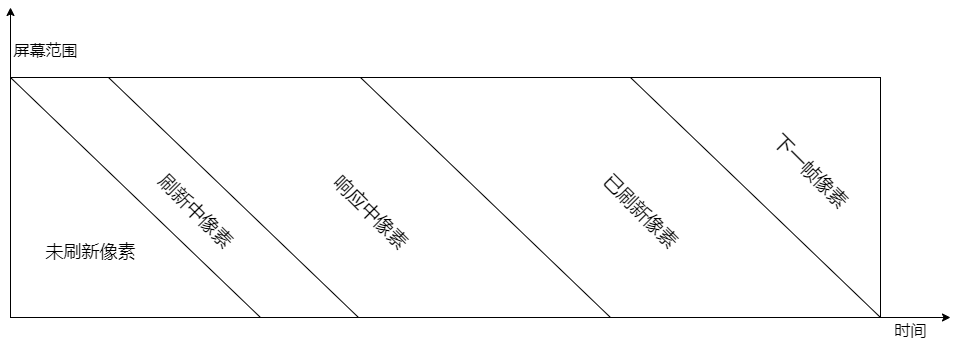
\includegraphics[scale=0.4]{figures/HW/Cap_Pt.png}
\caption{摄像头捕获的显示器刷新过程}
\end{figure}

显示器的面板详细属性参见附录A。

\subsection{摄像头与镜头}

解码端的摄像头用于拍摄展示后的二维码。摄像头的摄像频率不得低于60FPS,最高速率不设上限,但必须不影响功能的实现。摄像头应采用标准的网口或者USB接线传输数据,数据传输的带宽应当能够支持最高速拍摄时的数据速率。内部如有采用独立开发的接口的,必须提供合适的转接层,保证普通的计算机能直接通过网口或USB接线连接上摄像头。

需要调节摄像头的一系列参数从而得到屏幕图像的清晰图案。具体参数包括:光圈、感光度、曝光时间、增益、白平衡。摄像头所能拍摄的分辨率决定了拍摄图像对原始屏幕输出的解析能力,帧率决定了对屏幕图像的获取速度。二者直接制约接收端的接收带宽。

假定屏幕刷新率120FPS,则每1/120=0.0083=8.3ms,屏幕刷新一次。考虑到屏幕有响应时间(前一帧淡出,后一帧淡入),考虑2ms的情况(实际会有所偏差),屏幕的图像特性如图5.2所示。

\begin{figure}[!htbp]
\centering
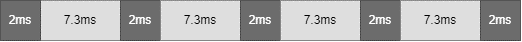
\includegraphics[scale=1]{figures/HW/Rf_Model.png}
\caption{显示器刷新模型}
\end{figure}

显然我们不希望在红色区的响应时间内拍照,因此就需要Lock-in同步。然而,也可以通过如下的两个逻辑解同步:

1.如果落在响应时间内,算法要能认识到这一点并抛弃一帧

2.下一帧一定落在本帧的非响应时间内

第一点,可以用纯色定位块解决。因为8张二维码不会堆满整个屏幕,所以我们可以在某一个区域放置纯色的定位块。接下来,我们为连续的三帧分别给上红绿蓝三种纯色定位块,称之为红帧、绿帧和蓝帧。考虑相机现在拍摄完红帧,这样,算法知道下一帧是绿帧。如果屏幕现在处于响应时间,定位纯色块要么是暗淡的灰色,要么是红绿之间的黄色,总之不会是纯绿色。因此,按照某种绿色阈值,可以检测并抛弃一帧。

第二点,如果我们使用150FPS的相机,则每1/150=0.0066=6.6ms,拍摄一张照片。考虑拍照时间落在响应时间内的两种极限情况(黄色和绿色标出),下一帧都一定会落在本帧的非响应时间内,从而得到正确的成像。摄像头采集的模型如图5.3所示。

\begin{figure}[!htbp]
\centering
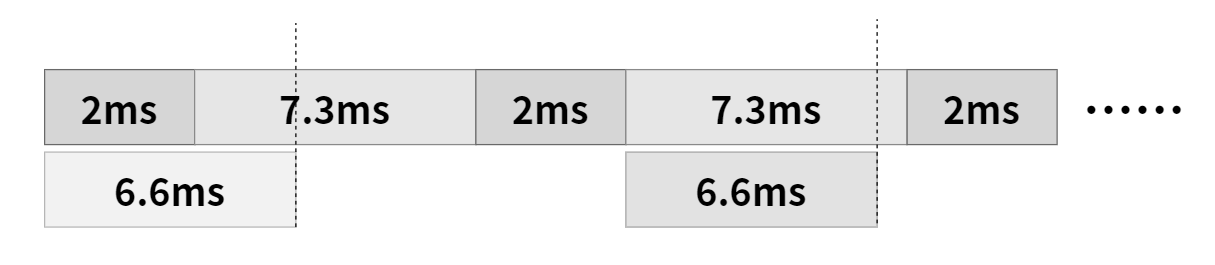
\includegraphics[scale=0.4]{figures/HW/Cap_Md.png}
\caption{摄像头采集模型}
\end{figure}

项目中摄像头采用Teledyne Lumenera Lt-C1950 Pregius Global Shutter CMOS USB3 Camera作为首选摄像头,其提供了1936 X 1216分辨率(230万像素)下162FPS高速实时图像传出。外形尺寸为45毫米x 45毫米x 36.1毫米,较为小巧,满足设计需求。

\begin{figure}[!htbp]
\centering
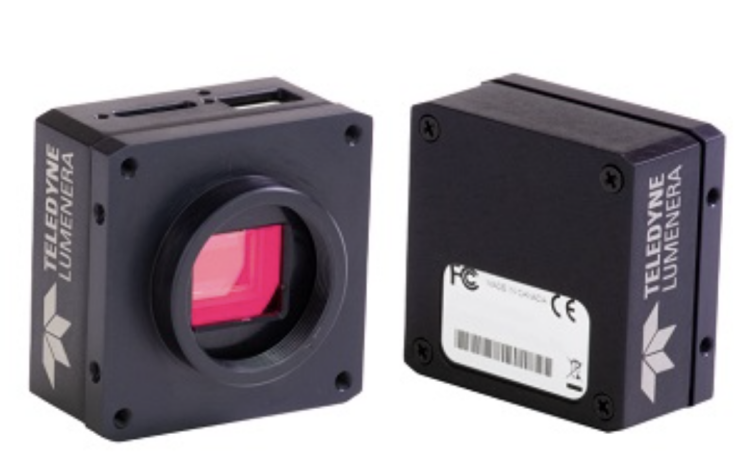
\includegraphics[scale=0.6]{figures/HW/LTC1950.png}
\caption{Lt-C1950摄像头}
\end{figure}

镜头的基本功能是光线转换(调制)。在视觉系统中,镜头的主要功能是将目标成像于相机的CMOS或是CCD上。镜头的好坏直接影响到系统的整体性能,合理选择与安装镜头是视觉系统设计与实施的一个重要组成部分。\cite{郑新宇0基于视觉检测的对位贴合系统设计与应用}

定焦镜头的主要调节参数为焦距与光圈。焦距越小,景深越大,畸变越大,渐晕现象越严重,使像差边缘的照度降低; 光圈越大,图像亮度越高,景深越小。\cite{刘混海2009基于机器视觉的集成芯片基板定位技术研究}

使用焦距小的镜头可以帮助减小整套光学传输模块的尺寸,但代价是获得的图像将有更明显的鱼眼效应与暗角。

项目中采用的镜头为500万像素1/1.8英寸VM0420MP5 4mm C口镜头。

\begin{figure}[!htbp]
\centering
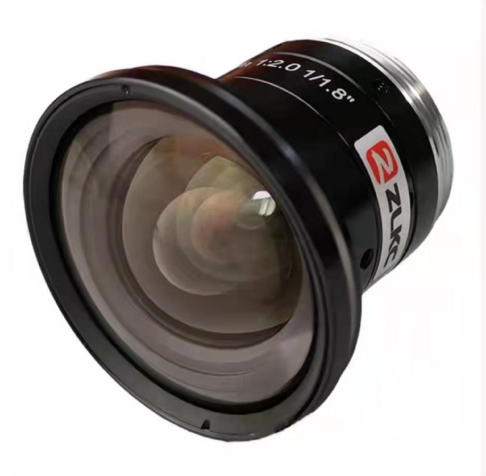
\includegraphics[scale=1.4]{figures/HW/VM0420MP5.png}
\caption{VM0420MP5镜头}
\end{figure}

受制于摄像头与屏幕之间的距离因素,一个摄像头无法捕捉到整个屏幕的完整画面。在本项目中使用两个独立摄像头拍摄同一块屏幕的不同区域。

\subsection{机架}

摄像头与屏幕固定在主承载支架上,保证摄像头与屏幕在工况下相对位置不发生变化。摄像头可以通过可靠的夹具夹持,显示器可以使用符合VESA标准的支架进行固定。主承载支架应当具有减震与避震措施,避免微振动对图像识别造成的影响。摄像头与解码服务器的数据线连接需要使用可靠的锁止装置,如果使用USB外形的接口,应当附加数据线与摄像头本体的锁扣链接;如果使用RJ-45外形的接口,需要确保水晶头的锁定可靠性。显示器与编码服务器的连接同样需要保证可靠性。VGA与DVI不足以承受系统所需要的显示带宽,故不使用。应当使用附加锁扣装置的HDMI数据线或者全尺寸DP接口的数据线(全尺寸DP接口自带锁止装置)。镜头可以通过C口连接到摄像头。如果采用定焦摄像头,则镜头的对焦转盘与光圈转盘应当安装有限位器,保持焦距与光圈的固定。

为避免环境光对系统运行产生的干扰,整个光学传输模块需要有完整的不透光蒙壳。蒙壳内侧(即光学传输模块运行的一侧)需要使用深色哑光材质,使得蒙壳自身的干扰降到最低。蒙壳内需要有一定的热量交换途径,防止摄像头与显示屏超出工作温度。如果采用风冷的方式,需要安装额外的空气滤清装置避免外部异物入侵到蒙壳内。机箱整体的尺寸(单位:mm)约为470(w)*800(l)*350(h),机箱内部的设计以及真实硬件如图5.6与图5.7所示。

\begin{figure}[!htbp]
\centering
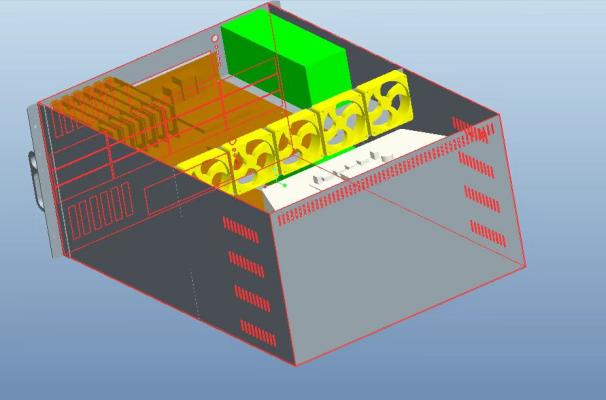
\includegraphics[scale=1.6]{figures/HW/Design.png}
\caption{服务器设计}
\end{figure}

\begin{figure}[!htbp]
\centering
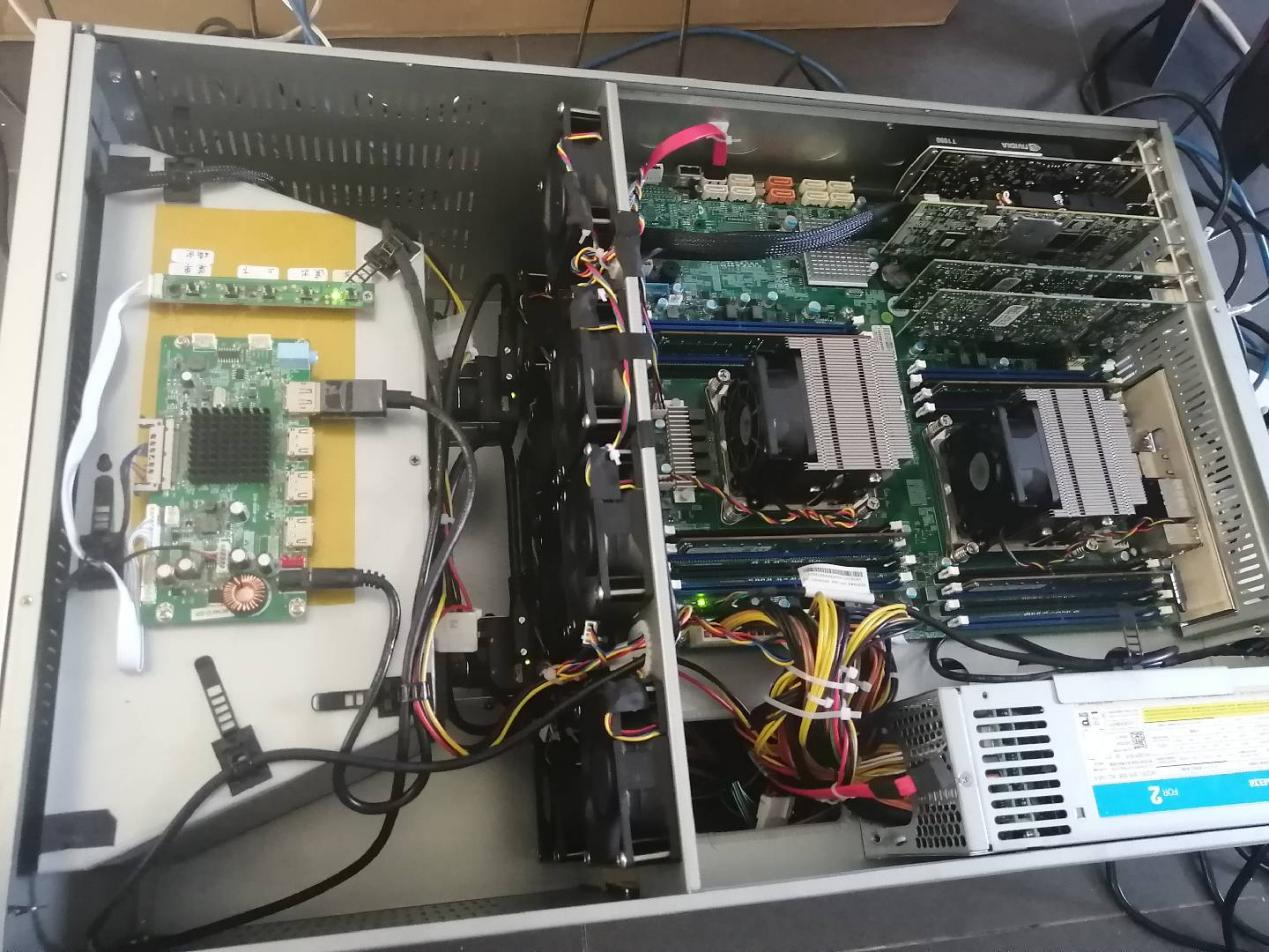
\includegraphics[scale=1]{figures/HW/Real_HW.png}
\caption{服务器硬件}
\end{figure}

服务器的硬件参数如表5.1,表5.2所示

\begin{table}[htb]
  \centering
  \begin{minipage}[t]{0.8\linewidth} 
  \caption[硬件参数]{硬件参数}
    \begin{tabularx}{\linewidth}{lX}
      \toprule[1.5pt]
      {\heiti 技术参数} & {\heiti 指标} \\\midrule[1pt]
      CPU    & INTEL E5 2699V4 *4 \\
      GPU    & NVIDIA T1000*1  NVIDIA T300*1 \\
      RAM    & 2*4*32GB \\
      存储   & 2*2*1000GB SSD RAID1系统盘,2*4*6TB HDD RAID5数据盘 \\
      网络接口    & 8*RJ45 千兆以太网网口 \\
      管理接口    & 2*RJ45 千兆以太网接口 \\
      USB    & 4*USB2.0 4*USB3.2Gen1 \\
      \bottomrule[1.5pt]
    \end{tabularx}
  \end{minipage}
\end{table}

\begin{table}[htb]
  \centering
  \begin{minipage}[t]{0.8\linewidth} 
  \caption[物理与电气特性]{物理与电气特性}
    \begin{tabularx}{\linewidth}{lX}
      \toprule[1.5pt]
      {\heiti 技术参数} & {\heiti 指标} \\\midrule[1pt]
      输入电源    & 100-240V 50-60Hz AC \\
      多电源输入    & 双电源冗余 \\
      功率    & 550W*2 \\
      过载与冗余保护  & 支持 \\
      尺寸(WxDxH) & 444*750*250mm \\
      重量(kg) & 50 kg \\
      散热设计 & 风冷 \\
      安装方式 & 19英寸6U机架 \\
      工作环境 & -10℃ ~ +40℃ ,5\% ~ 90\%无凝结 \\
      存储温度 & -20℃ ~ +60℃ ,5\% ~ 95\%非凝结 \\
      IP防护等级 & IP30 \\
      \bottomrule[1.5pt]
    \end{tabularx}
  \end{minipage}
\end{table}

\section{周边控制组件}

在有数据传输的能力之后,我们还需要对整个系统进行一定程度的控制,以更好地满足业务上的需求。

\subsection{网络与时间模块}

网络模块提供了配置系统网口,驱动Socket程序的能力。

网络模块提供了可以直接操纵系统级别网口配置的能力,在用户需要重新配置网络环境时,通过web应用或修改数据库的方式将配置文件存入MySQL的配置表中,发出网络配置指令后,网络模块会生成新的yaml配置文件,使用NetPlan的接口将新的配置作用于NetworkManager,然后对系统的配置作出修改。网络模块同时支持对ICMP报文的处理规则应用。

网络模块旨在提供易用的、即时生效的、重启不改变的网络环境配置,为配置静态IP、禁止ping服务等需求提供服务。网络模块生效的实现流程如图5.8所示。

\begin{figure}[!htbp]
\centering
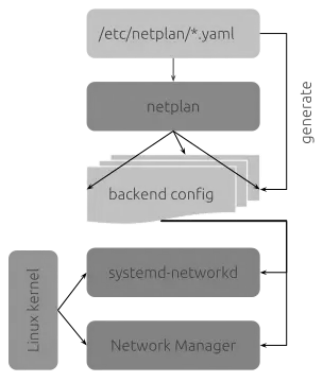
\includegraphics[scale=1]{figures/HW/N1.png}
\caption{网络配置流程}
\end{figure}

本系统提供NTP在不连接外网的情况下提供可靠的时间服务。

网络时间协议NTP用来使客户端和服务器之间进行时钟同步,提供高精准度的时间校正。NTP依赖从客户端到服务器的往返延迟delay,客户端与服务端之间的时间差offset来计算调整自己的时钟,实现与NTP服务器的时钟同步。

\subsection{IP白名单模块}

IP白名单模块提供了传输机别的基础安全机制,使用白名单方式保证传输的安全性。

对于编码侧与解码侧,IP白名单分别作用于两侧的Socket程序,只接受白名单IP发送的数据,只将数据发送给白名单内的IP。IP白名单存储允许连接的IP地址,在建立连接时检查来源地址/目标地址是否在白名单中,而后允许或者拒绝连接。

编码端的IP白名单检查发生在socket连接建立的过程中。对于发送到编码器的TCP或UDP请求,可以获知来源的IP地址,如果IP地址不在白名单中则直接断开当前连接。解码端的IP白名单发生在socket连接建立之前。由于总是由解码器进行连接的发起,对于不在IP白名单内的目的地址,不会尝试进行连接的建立。处理流程如图5.9所示。

\begin{figure}[!htbp]
\centering
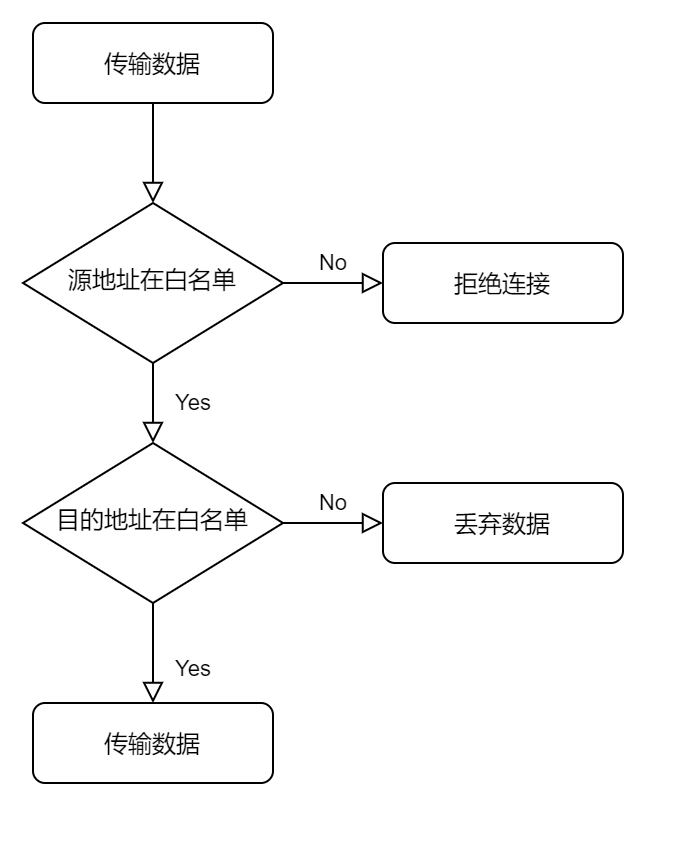
\includegraphics[scale=0.4]{figures/HW/N2.png}
\caption{IP白名单}
\end{figure}

IP白名单模块提供IP白名单的增删改查功能。通过该模块,用户可以便捷的对IP白名单进行各种必需操作,并实时的反映在整个传输系统上。IP白名单为单向隔离系统提供传输级别的IP地址过滤,是系统安全性的重要组成部分。

\subsection{用户模块}

本产品支持三权分立,内置配置员、审计员、管理员三个用户。

配置员:用于网络与用户配置。

审计员:用于事件日志审计。

系统管理员:用于系统管理。

通过用户模块,可以完成用户名单的增删改查工作,可以根据用户名与密码正确的进行用户的验证,可以在连续多次密码错误时对账号进行冻结,可以做到冻结时长与密码错误次数的联动,可以在超出冻结时长后自动对用户进行解冻,可以手动的对用户进行解冻,对不同权限的用户可以正确的接收、拒绝对应的操作。

本项目基于RBAC(基于角色的权限控制)模型进行权限管理。在本系统中,共预制有配置、审计、管理三种角色。不同的角色对应了不同的权限。

系统支持子菜单级别的用户管理。通过用户管理功能,可以创建若干角色并分配权限,创建用户时可以直接授权该角色的权限。对于已经创建的用户,可以进行修改与删除操作,支持修改的内容包括帐号、密码、权限等。

项目采用帐户密码认证+jwt方式验证用户的登录状态,token的失效期为1小时。所有前端请求会经过拦截器,再由后端验证token。用户在登录界面成功登录后 获取token,验证权限,而后用相应权限访问对应接口获得数据或者执行操作。Token采用SHA256算法加密。在无token、token过期、用户验证错误等情况下,会拒绝用户所做查询与操作。通过用户认证机制,可以依据权限做用户操作加以限制。

为了防止恶意使用者通过暴力枚举的方式破解用户密码,在短时间连续多次密码错误后会对用户进行冻结。在用户连续3次密码错误后,每一次失败的登录尝试会将账户的冻结时间累加3分钟。在冻结时间超时后,账户会自动解冻。管理员亦可以手动对指定的账户进行解冻操作。

\subsection{日志、数据缓存与流量统计}

本系统提供多种日志记录,提供完整的数据缓存以及持久化,提供基于缓存数据的流量统计。可以依照时间、分类、级别、关键词准确的查询对应的日志项,各个系统的关键操作可以被正确的记录到日志库中。

系统日志记录系统级别操作日志,包括NTP操作,端口初始化等。通过查询或审计系统日志,可以对系统运行状态以及历史操作进行审计。

警告日志记录系统运行时出现的各种错误情况,包括系统内部的传输错误、目的地址不可达、文件模式不符合等。

登录日志记录用户的登录操作,包括登录成功与登录失败的记录,便于管理员判断用户行为模式,及时对异常情况做出操作。

操作日志记录对于系统所做的一系列配置操作,包括网络配置、用户配置、IP白名单配置等。用户所做出的重要操作均会被记录于操作日志中。

由于系统存在严格的单向性,对于解码器出现的错误,编码器完全无法获知,使得整个系统无法提供严格意义的可靠传输,只能提供尽最大可能的无差错传输。如果出现问题,需要借助外力介入进行恢复或重传,对于时间段内的数据,将它们进行暂存是一种较好的方式。但是对于成功的传输,系统亦无法得知其具体的传输情况。因而采取对所有的传输全部暂存的方式。

对于所有的传输,基于Linux系统“一切皆文件”与单向网闸的设计,接受到的数据流会首先以文件形式进行缓存、传输,对于传输完成的文件,会根据传输信息与传输状态,将文件移动到对应的备份路径下进行保留。如果后期需要恢复文件,可以根据传输的网口号、协议、传输时间进行对应的查找。

所有发送数据的内容部分,会以原始二进制形式进行数据备份。存储时不指定特定格式,统一作为比特流处理,存储为无后缀元文件。存储以入库网口-协议-精确到纳秒的传输发生时间作为文件名,便于数据的查找与恢复。记录保存6个月。

在流量统计模块中,可以查看流量总览和设备流量趋势。

流量统计主要包含主要包含了流量总览和端口流量两个部分。流量总览显示设备总的流量数据和根据协议分类汇总的数据。端口流量按端口号显示流量数据。

流量总览可以依据协议,以分钟或小时作为时间单位显示过去10个时间段的传输流量以及传输条数。端口总览可以依据端口号,以分钟或小时作为时间单位显示过去10个时间段的传输流量以及传输条数。

传输流量可以记录每一个传输的发包数以及传输条数,传输流量可以根据时间段、协议、网口号、IP、端口等,显示符合内容的每一条传输的传输数据量以及发包数,一并包括精确到毫秒的传输时间、传输的IP地址与端口号、协议等一系列审计相关内容。

\section{用户界面}

在本系统中,还提供易于操作的Web管理界面,对整个传输系统进行配置。

项目服务端由Django4构建,使用MySQL作为数据库,并用Redis做一层缓存。项目前端由VUE实现。具体的前后端接口列表见附录B。

\subsection{登录与用户管理}

用户访问编码器的前端地址会被自动路由至登录页面,在编码器的登录页面有用户的登录操作的接口,分别为编码器用户的用户名和密码。其中编码器用户的账号分为管理员权限,审计权限和配置权限。在登录界面没有用户的注册功能,用户的账号的密码为拥有管理权限的管理员账号使用添加用户功能完成。

登录界面分为登录错误和登录成功两种提示,当登录成功时,用户会被自动跳转至该编码器登录用户所对应权限可访问的功能页面。每个用户在密码输入和用户名不匹配时会提示登录错误,每个用户的登录错误次数超过三次时,该账户会被锁定,用户需要联系在系统中管理员权限的账号持有者,通过管理员权限中的解冻锁定账户的功能重新获得该账户的使用权限。登录界面如图5.10所示。

\begin{figure}[!htbp]
\centering

\includegraphics[scale=1]{figures/HW/N3.png}
\caption{用户登录}
\end{figure}

用户配置可以由拥有管理员权限的用户更改解码器中用户的信息。该页面包括以下功能:用户添加,修改用户信息和删除用户。在该页面展示系统中所有用户的信息。包括用户的序号。用户姓名、该用户的权限、该账号的状态、该用户的密码、该用户的账号上述信息。配置界面如图5.11所示。

\begin{figure}[!htbp]
\centering
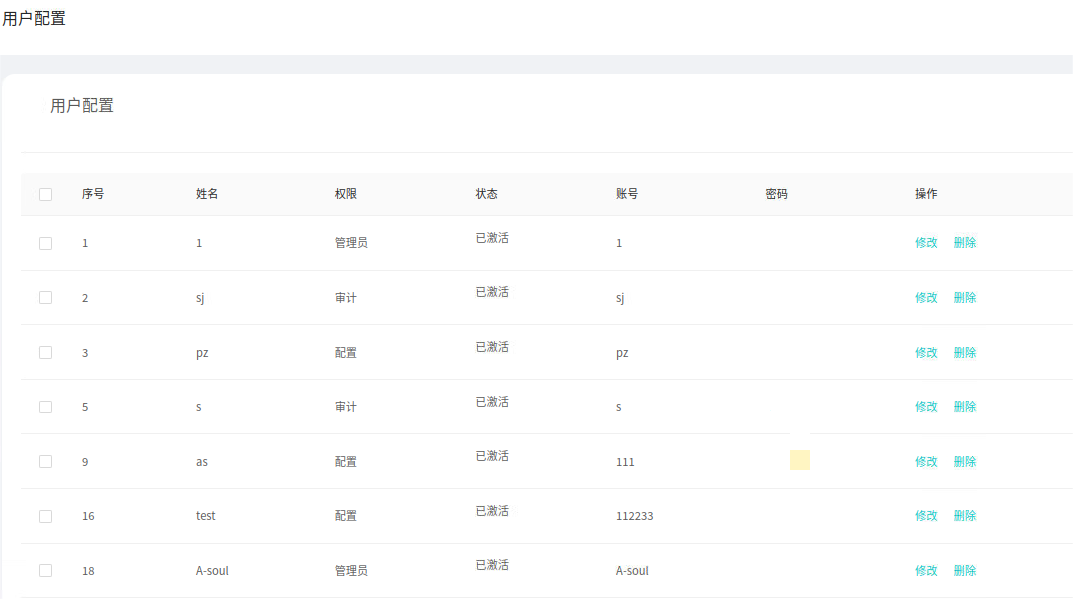
\includegraphics[scale=0.5]{figures/HW/N4.png}
\caption{用户管理}
\end{figure}

\subsection{展示页}

传输展示由展示传输统计和展示产品信息以及展示设备状态等三部分功能完成,系统状态均为实时更新。通过展示页面可以使用户更好的对系统的运行状况进行了解。

编码器传输统计分成两部分主要功能,别分为分开统计编码器的实时传输数据量,和实时传输数据的条数,而统计的功能又分为每小时的数据统计和每分钟的数据统计。同时系统可以选择不同的网口展示来自每个网口的单独统计数据,该网口由实际的接入编码器的网口控制,网口信息可以在网络管理章节中查看,并定义。

本页面所展示的所有数据都分为监听前七个时刻的数据,分别由小时和分钟两种请求方式,在本页面中两个矩形框的右上角分别设有两个下拉选项,该选项框可操控显示矩形框中所请求的实时传输数据为分钟时刻/小时时刻,矩形框内会根据所请求的数据进行图形绘制和数据可视化。

编码器的展示数据功能分别为TCP协议和UDP协议分开展示,图5.12中该页面的蓝色矩形展示框为TCP数据展示界面,绿色矩形展示框为UDP数据展示界面。

\begin{figure}[!htbp]
\centering
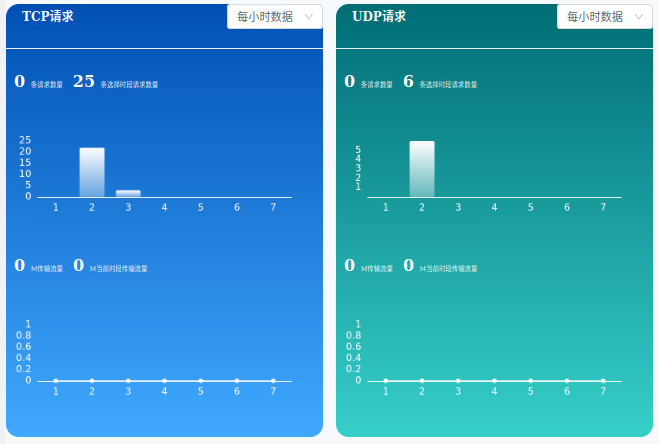
\includegraphics[scale=1]{figures/HW/N5.png}
\caption{数据展示}
\end{figure}

蓝色矩形的上方半部为请求TCP数据的条数的统计展示,分别展示前七个时刻的统计TCP数据,并绘制折线图和柱状图。在所展示的图形的上方为当前一个时刻的TCP数据和前七个时刻TCP数据的总和。蓝色矩形的下方半部为请求TCP数据的流量大小的统计展示,分别展示前七个时刻的统计数据,并绘制折线图和柱状图。在所展示的图形的上方为当前一个时刻的数据和前七个时刻数据的总和。

绿色矩形的上方半部为请求UDP数据的条数的统计展示,分别展示前七个时刻的统计UDP数据,并绘制折线图和柱状图。在所展示的图形的上方为当前一个时刻的UDP数据和前七个时刻UDP数据的总和。绿色矩形的下方半部为请求UDP数据的流量大小的统计展示,分别展示前七个时刻的统计数据,并绘制折线图和柱状图。在所展示的图形的上方为当前一个时刻的数据和前七个时刻数据的总和。

设备状态展示分为展示解码器CPU的状态,内存状态和硬盘状态。该三个硬件设备的状态为每秒钟实时更新的设备状态,如图5.13所示。

\begin{figure}[!htbp]
\centering
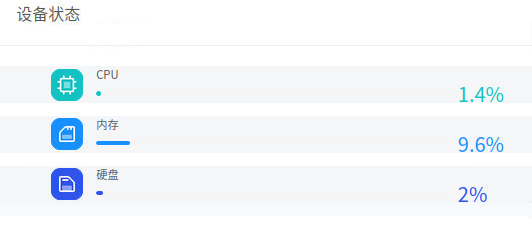
\includegraphics[scale=1]{figures/HW/N6.png}
\caption{设备状态}
\end{figure}

\subsection{网络管理}

网络配置模块提供易用的网络配置抽象,使得用户可以较为便捷的做出系统级别的网络配置更改。

在编码器管理口配置中,管理口的参数分为,IP,网口,子网掩码,网关,web服务,ping服务等属性。编码器的所有管理口的配置将会展示在该页面。在该页面的管理口展示中,拥有网络管理配置权限的用户可以通过展示界面的编辑按钮来修改管理口的配置。管理口的配置界面如图5.14所示。

\begin{figure}[!htbp]
\centering
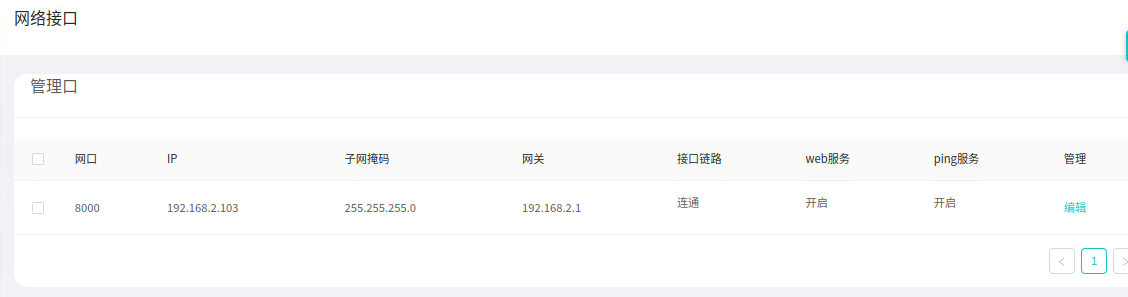
\includegraphics[scale=0.6]{figures/HW/N7.png}
\caption{管理口管理}
\end{figure}

在编码器业务口配置中,业务口的参数分为,网口,入口端口,子网掩码,网关,协等上属性。编码器的所有业务口的配置将会展示在该页面。在该页面的业务口展示中,拥有网络管理配置权限的用户可以通过展示界面的编辑按钮来修改业务口的配置。业务口配置界面如图5.15所示。

\begin{figure}[!htbp]
\centering
\includegraphics[scale=0.6]{figures/HW/N8.png}
\caption{业务口管理}
\end{figure}

在解码器管理口配置中,管理口的参数分为,IP,网口,子网掩码,网关,web服务,ping服务等属性。解码器的所有管理口的配置将会展示在该页面。在该页面的管理口展示中,拥有网络管理配置权限的用户可以通过展示界面的编辑按钮来修改管理口的配置。管理口的配置界面如图5.16所示。

\begin{figure}[!htbp]
\centering
\includegraphics[scale=0.6]{figures/HW/N9.png}
\caption{管理口管理}
\end{figure}

在解码器网口配置中,网口的参数分为,IP,网口,子网掩码,网关,以上属性。解码器的所有网口的配置将会展示在该页面,网口的展示效果如图5.17所示。

\begin{figure}[!htbp]
\centering
\includegraphics[scale=0.6]{figures/HW/N10.png}
\caption{网口管理}
\end{figure}

在解码器业务口配置中,业务口的参数分为,网口,出口网口,目的IP,目的端口,目的IP协议,子网掩码,网关等属性。解码器的所有业务口的配置将会展示在该页面,在该页面的业务口展示中,拥有网络管理配置权限的用户可以通过展示界面的编辑按钮来修改业务口的配置。业务口的展示效果如图5.18所示。

\begin{figure}[!htbp]
\centering
\includegraphics[scale=0.6]{figures/HW/N11.png}
\caption{业务口管理}
\end{figure}

业务口的配置目的是形成一张路由表,完成单向网闸的端口映射以及转发。各个配置的关系如图5.19所示。

\begin{figure}[!htbp]
\centering
\includegraphics[scale=0.4]{figures/HW/N12.png}
\caption{各个配置之间的关系}
\end{figure}

\subsection{数据缓存与日志}

通过数据缓存和日志模块,我们可以对系统传输的内容以及发生的时间进行追溯,保证系统的安全性,及时发现系统漏洞。

数据缓存界面可以查看详细的历史传输数据。数据缓存页面分为查询部分和数据展示部分。查询部分为图中的上半部分,用户可通过输入源IP、目的IP、使用传输协议、开始时间和结束时间五个参数来查询解码器系统中的历史传输数据。其中源IP、目的IP需要用户手动输入,所使用传输协议是一个下拉框,用户可选择查看TCP协议和UDP协议,开始时间和结束时间是通过日历选择实现,用户可以通过一个下拉日历选择需要查询的数据时间跨度。用户也可以通过日历中的此刻按钮来选择操作时间为需要的时间。查询成功后系统会提示查询成功。

数据查询接口为模糊查询,这意味着用户不需要输入全部的属性作为查询的参数,可以通过输入部分属性进行查询。例如,用户仅输入源IP和目的IP这两个查询参数,这意味着得到的结果是满足这两个查询参数的所有数据。此处的重制按钮可以清除用户已输入的查询参数。查询界面如图5.20所示。

\begin{figure}[!htbp]
\centering
\includegraphics[scale=0.6]{figures/HW/N13.png}
\caption{查询界面}
\end{figure}

编码器的日志查询功能可以通过输入查询参数获得系统中已有的日志列表。其中可供用户选择的参数为,查询日志的关键字、日志的级别、查询的开始时间和查询的结束时间。日志页面如图5.21所示。

\begin{figure}[!htbp]
\centering
\includegraphics[scale=0.6]{figures/HW/N14.png}
\caption{日志页}
\end{figure}

\section{本章小结}

在本章,我们介绍了与前文提到的基于二维码的传输系统相配套的硬件设备以及控制模块,并且实现了一套可用于用户交互的前后端管理系统。到此为止,我们真正的实现了一台符合工控需求,可以用做单向隔离系统的网闸设备,并且可以在此基础上进行信息的传递。

% !Mode:: "TeX:UTF-8"
\begin{conclusion}

本项目提出了一种复杂环境下的高效自适应二维码编解码方案,可以有效的抵抗画面发生的一定程度的形变、色彩偏移,并且保证传输内容的高度可靠性。整套解决方案没有高级计算机图形库与复杂神经网络的参与,并且编解码效率非常高。

基于复杂环境下的高效自适应二维码编解码技术,本项目完成了一套基于自定义二维码与图像识别技术的单向网闸,研究了一套基于离散二维码的高可靠、可纠错的文件传输协议,并基于此协议实现了基于二维码的文件单向传输信道。

在传输的过程中,针对传输的内容进行压缩,调节二维码版本,对写入过程进行优化,调节纠错参数,实现了没有反向确认信道情况下保证99.999\%可靠性的,在传输工况下可能传输的文字内容的情况下(数据经过压缩)传输速率达到24Mbps的通信信道。

设计了一套适用于本系统的,与标准机架兼容的硬件设备,并且能与软件协同工作,工作状态符合预期。

在中国核工业集团福清核电站部署了包括硬件、软件在内的整套传输系统,正在进行长期稳定性测试。

\end{conclusion}

\bibliography{reference/refs}

\backmatter
\begin{appendix}
\chapter{显示器面板参数}
论文中提及的显示器面板参数。

在面板的参数中,我们重点关注其尺寸及PPI、面板亮度、工作频率、面板类型以及反应时间。

\begin{figure}[!htbp]
\centering
\includegraphics[scale=0.5]{figures/HW/PA_A.png}
\caption{AOCQ27G2S-K7E面板}
\end{figure}

\begin{figure}[!htbp]
\centering
\includegraphics[scale=0.8]{figures/HW/PA_B.png}
\caption{BENQXL2546K面板}
\end{figure}

\begin{figure}[!htbp]
\centering
\includegraphics[scale=0.8]{figures/HW/PA_C.png}
\caption{BOENE156FHM-NZ1面板}
\end{figure}

\chapter{前后端接口列表}
前后端对接所依赖的接口列表。

NTP相关

同步NTP时间
0.0.0.0:8000/DecoderBack/NtpSync/

参数:
ip: NTP服务器IP或URL(ntp.aliyun.com),
time-zone: 时区('Asia/Shanghai'),
返回:
isOk: 执行状况(True/False),

网络接口相关

获取管理接口配置与状态
0.0.0.0:8000/DecoderBack/GetManagePortConfig/

参数:无参数

返回:
isOk: 执行状况(True/False),
managemenmtPortConfig: 管理接口配置,

获取业务接口配置
0.0.0.0:8000/DecoderBack/GetDataPortConfig/

参数:无参数,

返回:
isOk: 执行状况(True/False),
dataPortConfig: 业务接口配置,

获取网口配置
0.0.0.0:8000/DecoderBack/GetEthernetPortConfig/

参数:无参数,

返回:
isOk: 执行状况(True/False),
dataPortConfig: 网口配置,

编辑管理接口配置[仅数据库]
0.0.0.0:8000/DecoderBack/EditManagePortConfig/

参数:
ip,
port,
subnet-mask 子网掩码,
gateway 网关,
status 链路状态(bool),
web-running Web服务运行状态(bool),
ping-allowance 允许ping(bool),

返回:
操作状态,

编辑业务接口配置[仅数据库]
0.0.0.0:8000/DecoderBack/EditDataPortConfig/

参数:
access 对应编码端网口,
exit-access 对应解码端网口,
exit-port 出口端口,
target-ip = 目的ip,
target-port = 目的端口,
protocol = 协议,

返回:
操作状态,

编辑网口配置[仅数据库]
0.0.0.0:8000/DecoderBack/EditEthernetPortConfig/

参数:
ip 网口IP,
access 网口号,
subnet-mask 子网掩码,
gateway 网关,

返回:
操作状态,
系统状态相关,

获取系统状态
0.0.0.0:8000/DecoderBack/GetSystemStatus/

参数:无参数,

返回:CPU, RAM,存储,

IP白名单相关

获取IP白名单列表
0.0.0.0:8000/DecoderBack/GetIpWhiteList/

参数:
offset 日志展示起始位置,[offset : offset+20],

返回:
IP白名单列表,

新增IP白名单项
0.0.0.0:8000/DecoderBack/AddIpWhiteList/

参数:
ip: 新增IP,

返回:
操作状态,

删除IP白名单项
0.0.0.0:8000/DecoderBack/DelIpWhiteList/

参数:
id: 白名单序列号(由GetIpWhiteList/返回),

返回:
操作状态,

编辑IP白名单项
0.0.0.0:8000/DecoderBack/EditIpWhiteList/

参数:
ip: 新增IP,
id: 白名单序列号(由GetIpWhiteList/返回),

返回:
操作状态,

用户相关

新增用户
0.0.0.0:8000/DecoderBack/AddUser/

参数:
account,
name,
password,
authority 权限 1=管理员 2=配置 3=审计,
active 活跃状态,

返回:
操作状态,

删除用户
0.0.0.0:8000/DecoderBack/DelUser/

参数:
account,

返回:
操作状态,

编辑用户
0.0.0.0:8000/DecoderBack/EditUser/

参数:
id,
account,
name,
password,
authority 权限 1=管理员 2=配置 3=审计,

返回:
操作状态,

获取用户列表
0.0.0.0:8000/DecoderBack/GetUserList/

参数:无参数,

返回:
用户列表,

获取用户信息(获取用户列表的单用户版本)
0.0.0.0:8000/DecoderBack/GetUserInfo/

参数:
account: 用户帐号,

返回:用户信息,

验证登录
0.0.0.0:8000/DecoderBack/AuthUser/

参数:
account: 用户帐号,
password: 用户密码 ,

返回:
能否登录,是否可管理,是否可查看,是否被冻结,

获取冻结名单
0.0.0.0:8000/DecoderBack/GetFreezingUserList/

返回:
冻结用户信息,

解冻用户
0.0.0.0:8000/DecoderBack/UnfreezeUser/

参数:
account: 用户帐号,

返回:
操作结果,

日志相关

获取日志列表
0.0.0.0:8000/DecoderBack/GetLog/

参数:
time-start: 筛选开始时间 2022-06-11 12:00:00[.123456],
time-end: 筛选结束时间,
classify: 日志类别(system, user, operation, warning)(''=All),
level: 日志级别(info, warning,) [''=all],
content 内容关键字筛选(''=All),
offset 日志展示起始位置,[offset : offset+20],

返回:
totalLength: 日志总条数,
Log: 可迭代,[[<时间>, <级别>, <内容>], [], []...],

传输相关

获取传输列表
0.0.0.0:8000/DecoderBack/GetTransferList/

参数:
time-start: 筛选开始时间,
time-end: 筛选结束时间,
exit-ip: 出口IP(''=All),
target-ip 目的IP(''=All),
protocol: 协议(''=All),
offset 日志展示起始位置,[offset : offset+20],

返回:
传输列表,

传输状态统计
0.0.0.0:8000/DecoderBack/GetTransferInfo/

参数:
time-start: 筛选开始时间,
time-end: 筛选结束时间,
Access: 网口选择(''=All),
protocol: 协议(''=All),

返回:
length: 数据条数,
size: 数据大小(字节数),

Token相关

Token会在AuthUser接口获得,这也是唯一一个无需token验证的接口。
在后续请求中,在Header部分加入Token,完成后续验证。

Token验证失败返回HTTP状态码401UnAuthorized

Messige释义:

No authenticate header:Header没有包含Authorization字段

Error authenticate header:Header包含Authorization字段,但无效或为空值

Token expired:token超过有效期限

Invalid token:无效的token

Unexpected token error:解析token时出现的其他错误

User no longer exist or token lost effiency:用户不再存在,或者被手动注销

Mismatched Authority: ManagementRight required:需要管理权限(但没有)

Mismatched Authority: AuditRight required:需要审计权限(但没有)

\end{appendix}

% 致谢
\begin{acknowledgement}

在本文写完之时,上文提到的“智能图像识别单向隔离装置”已经在中核福清核电站的机架上运行了数月。首先要感谢中核武汉核电运行技术股份有限公司的张登主任以及中核福清核电站信息文档处的梁浩科长在本项目的落实过程中基于的大力支持,使得本项目的最终落实成为了现实。

感谢张国荣高级工程师在本项目的硬件加工、组装过程中给予的帮助与支持。

感谢钟鸣宇学长、陈成学长在Rust语言编程、项目的核心架构编写上给予的意见与建议。

感谢金泓宇同学在项目的前后端编写中给予的帮助。

感谢上海大学开源社区提供的LaTeX模板,使本文的写作过程中避免了许多排版与格式的调整成本。

最后,尤其感谢项目导师武星教授对本人的精心指导。在本文的写作过程中,武星教授给予了在内容、排版、格式上的许多有用的建议,在项目的进行过程中的指导使项目的进行更加顺畅,避免了许多本可能出现的问题。

\begin{flushright}
顾骏杰\\
上海大学\\
2023年6月2日\\
\end{flushright}

\end{acknowledgement}


\includepdf[pages={1}]{back-cover.pdf} 

\end{document}
